\section{Introduction}


In the pursuit of better natural language interfaces with databases, Large Language Models (LLMs) have become the defacto standard for translating natural language questions into SQL queries.
LLMs, especially those not finetuned on target database schemas, require LLM prompts to include text-based schema knowledge representations in order to avoid confabulation of non-existent schema elements and to ensure generated SQL queries contain valid schema identifiers.
While including schema knowledge representations in prompts to modern LLMs is not a problem for moderately-sized schemas, some real-world databases including several enterprise resource planning systems, contain thousands of tables and tens of thousands of columns.
In these cases, schema knowledge representations that include supplemental information such as column and table descriptions can exceed even SoTA LLM context window limitations, which can significantly degrade or eliminate the ability of an LLM to generate valid SQL queries.

In addition to the hard constraint of context window limitations, even the newest LLMs are still susceptible to degraded information recall due to large inputs. 
This tendency is commonly referred to as the \emph{needle in a haystack} problem, that describes a model's ability (or failure) to retrieve information from input prompts~\cite{hsieh2024ruler}.
Although some recent large context models such as GPT4.1 claim to have successfully mitigated needle in a haystack-related errors, the ability of a model to perform more complex tasks more akin to determining the usefulness of a table or column to a natural language question, such as \emph{multi-round co-reference resolution} (MRCR)~\cite{vodrahalli2024michelangelolongcontextevaluations}, are still negatively affected by high token counts~\cite{openai2025gpt41}.

The idea of reducing schema representation in LLM prompts to improve LLM-based SQL generation has taken form in several high-ranking NL-to-SQL methods on recent benchmark submissions, and some recent analysis of LLM-based schema linking methods provides a mixed view of the costs and benefits of such approaches.
Our concurrent and complementary analysis of schema subsetting takes the body of schema research work even farther by asking two questions: 1) \emph{of the multiple existing schema subsetting methods, which one is ``the best'' and has the most positive impact on NL-to-SQL?} and 2) \emph{even though schema subsetting seems to have only a marginal effect (at best) on NL-to-SQL performance over smaller benchmark database schemas, what effect does it have on very large database schemas?} 

\paragraph{\textbf{Our Focus}}
In this paper, we extend the field of recent schema linking research by examining 7 real-world schema subsetting modules reproduced from NL-to-SQL project source code, and testing them over 3 benchmark datasets including Bird, the emergent Spider 2, and schema linking-focused SNAILS--making this the first work to evaluate real-world schema linking modules, using schema linking-focused performance and efficiency metrics, over very large database schemas.
Using the lessons learned from this analysis, we also present a prototype hybrid schema linking method which we call \PROJECTNAME{ }to motivate additional research toward more effective and efficient schema linking.

\paragraph{\textbf{Schema Subsetting (AKA Schema Linking)}}

Schema subsetting (also known as schema filtering, schema linking, structured grounding, or entity retrieval) is an approach used by many database NLIs to reduce schema knowledge size as a method for avoiding context window limitations and mitigating the needle in the haystack problem that can occur with very large prompts.
With LLM-based NL-to-SQL launching the usefulness of natural language interfaces (NLI) to databases into the realm of the practical, attempts to further improve the quality of SQL inference have begun to focus on sub-problems including schema linking.
Recent analysis of schema linking usefulness has produced mixed results.
On one hand, given an oracle (perfect) schema recall, decreasing the false positive rate (precision) generally improves NL-to-SQL generation for smaller open source LLMs~\cite{Katsogiannis-Meimarakis2026}.
On the other hand, schema linking proves to be less useful without oracle knowledge, and can even be detrimental to NL-to-SQL generation when the cost of omitting required tables and columns outweights the benefit of reduced schema representations in LLM prompts. 
This is primarily the case for the highest performing ``flagship'' LLMs~\cite{maamari2024deathschemalinkingtexttosql}.
Current schema linking methods and analysis has relied on the Bird~\cite{benchmark-bird} and Spider~\cite{benchmark-spider} benchmarks which have schema sizes smaller than many real-world systems.


\paragraph{\textbf{NL-to-SQL Benchmarks}}

The availability and difficulty of NL-to-SQL benchmarks have evolved at a pace relatively aligned with the advancement of NL-to-SQL systems.
BIRD~\cite{benchmark-spider} is currently the most active benchmark, and offers a level of complexity that has posed a challenge for the current generation of LLMs and systems to achieve human-level performance.
The BIRD benchmark consists of 95 databases, over 12,000 question-SQL pairs, and 37 domains. 
These data are split across a training, dev, and test set with the training and dev set available to the public.

Spider~\cite{benchmark-spider} was the most active NL-to-SQL benchmark at the beginning of the LLM-based NL-to-SQL era, and provides an interesting view of the associated advancement in NL-to-SQL capability over time.
Spider has since reached benchmark saturation, and Spider 2.0~\cite{benchmark-spider2} supersedes it as the newest NL-based database interaction benchmark, focusing on multi-step data retrieval over large and complex schemas.
Unlike its predecessors, Spider 2.0 does not provide dev or test set question-SQL pair data for model training.
Instead, the authors make a subset of the test data question-SQL pairs available (256 total) to assist developers with prompt design.
Spider 2.0 extends the set of target databases beyond Sqlite and also includes both Snowflake and BigQuery databases.

The SNAILS~\cite{benchmark-snails} project contains a benchmark dataset of 9 databases and 503 question-SQL pairs designed to represent real-world relational database schema design patterns including schema naming practices (defined as naturalness), schema size, and complex dependencies.

% Finetuned Language Models


% API-based frontier LLMs

% Multi-mode 

\paragraph{\textbf{Contributions}}
This paper makes the following contributions:

\begin{itemize}
  \item A schema subsetting-specific evaluation framework that isolates schema subsetting modules as independent processes.
  \item A reproduction and empirical analysis of 7 real-world schema subsetting modules from published code repositories.
  \item We present \PROJECTNAME: a subsetter prototype for improving NL-to-SQL over very large schemas.
  \item Extension of recent research of schema subsetting to very large schemas and discovery of both the usefulness and degradation of schema subsetting performance over these schemas.
\end{itemize}

% 
\section{Methodology}


To thoroughly evaluate multiple subsetting methods across multiple benchmarks, we create a modular object-oriented architecture to standardize interfaces between benchmarks, subsetting methods, evaluation processes, and NL-to-SQL generation.
The core of this approach is the schema data object, represented in our project as a Python object that can be transformed to DDL and JSON representations and is exclusively used as the representation of both full and subset schemas throughout the project codebase.

\subsection{Benchmarks}

\begin{table}
\caption{Schema size distribution for each benchmark dataset.}
\label{tab:benchmark-schema-sizes}
\begin{tabular}{llrrrr}
\toprule
Size & Columns & Bird & Snails & Spider2 & Total \\
\midrule
S & <100 & 9 & 1 & 34 & 44 \\
M & <1,000 & 2 & 6 & 43 & 51 \\
L & <2,500 & 0 & 1 & 10 & 11 \\
XL & <50,000 & 0 & 0 & 14 & 14 \\
XXL & <100,000 & 0 & 1 & 4 & 5 \\
\bottomrule
\end{tabular}
\end{table}


\paragraph{\textbf{Benchmark Data}}

To evalute subsetting methods against a diverse set of schemas, we retrofit the Spider2~\cite{benchmark-spider2}, SNAILS~\cite{benchmark-snails}, and Bird~\cite{benchmark-bird} NL-to-SQL benchmarks.
All benchmarks conform to the $\QUESTIONPAIR := <\QNL, \SQLGOLD>$ format, where NL questions are paired with a ground truth $\SQLGOLD$ used for evaluating correctness of subsetting method-generated $\SQLPRED$ queries.

Table~\ref{tab:benchmark-schema-sizes} summarizes the benchmark schemas in terms of 5 size categories based on the total number of columns in a schema.
The Bird dev set, the benchmark that appears most often in similar research, contains only small- and medium-sized schemas whereas the Snails and Spider 2 collections contain much larger schemas.
Schema size categorization enables a cross-benchmark evaluation of subsetting that prioritizes overall schema size over the source benchmark, which is important in subsetting evaluation because some methods are constrained by model input context limits that may render them useless in a particular size category.

\paragraph{\textbf{Benchmark Integration}}
The three benchmarks differ from each other in terms of how they perform schema representation, gold query and natural language question pairs formatting, and database storage and access.
We define an abstract NL to SQL object with standard function calls and iterators that serves as the super class to the individual benchmark sub-classes that wrap the underlying benchmark behaviors in a standardized interface. 
This approach allows us to perform online benchmark instantiation using a factory class and greatly increases the interchangeability of benchmarks in the subsetting evaluation and NL-to-SQL experiments.

\subsection{Schema Subsetting}
We modularize and abstract the schema subsetters in a similar fashion as the benchmark class.
Extracting the subsetting behavior from real-world NL-to-SQL systems varies in complexity by each system with some methods requiring more complex interfaces than others.
Regardless of underlying method complexity, we are able to apply a singular schema subsetter interface to each one, thus also making the subsetter modular and relatively ``easy'' to modify existing methods and experiment with new methods.
Schema subsetters take as input a benchmark question object that contains the associated schema object as well as a natural language question and return a subsetter result that contains a schema object (subset) and token usage data.

\subsection{NL-to-SQL Generation}
There are a variety of approaches to LLM-based NL-to-SQL generation, and the NL-to-SQL systems from which our evaluated subsetting modules employ an array of various post-subsetting techniques including zero-shot NL-to-SQL generation, error correction, few-shot example-based NL-to-SQL generation, and others.
To maintain consistency in evaluation between subsetting methods, we forego more complex NL-to-SQL techniques and instead use a zero-shot prompting approach that includes SQL generation instructions, the schema subset (represented serially as table: column 1, column 2, ..., column n), and additional evidence or hints relating to the schema if provided in the benchmark dataset.

We evaluate 7 LLMs from the OpenAI GPT~\cite{openai_gpt4.1_2024, openai2025gptoss120bgptoss20bmodel}, Meta Llama~\cite{grattafiori2024llama3herdmodels}, and Google Gemini~\cite{geminiteam2024gemini} model families.
We categorize the models into 3 classes: \emph{Flagship models} (GPT 4.1, Gemini 2.5 Pro), \emph{economy models} (GPT 4.1-Nano, Gemini 2.5 Flash, Gemini 2.5 Flash-Lite), and \emph{open source models} (Llama 3.3 70B Q8, GPT OSS 120B). 

We use the OpenAI and Google API libraries for flagship and economy model integration.
We host Llama 3.3 using Ollama on a dedicated server equipped with 2 AMD 9254 24-core processors, 541GB of system memory, and 2 NVIDIA A100 GPUs, with the model occupying 1 GPU.
We host GPT OSS 120B using vLLM on a dedicated server equipped with 2 AMD 9654 96-core processors, 1,623 GB of system memory, and 8 NVIDIA H100 GPUs, with the model occupying 4 GPUs.

\subsection{The \PROJECTNAME{ }Subsetter}

\begin{figure}
  \centering
  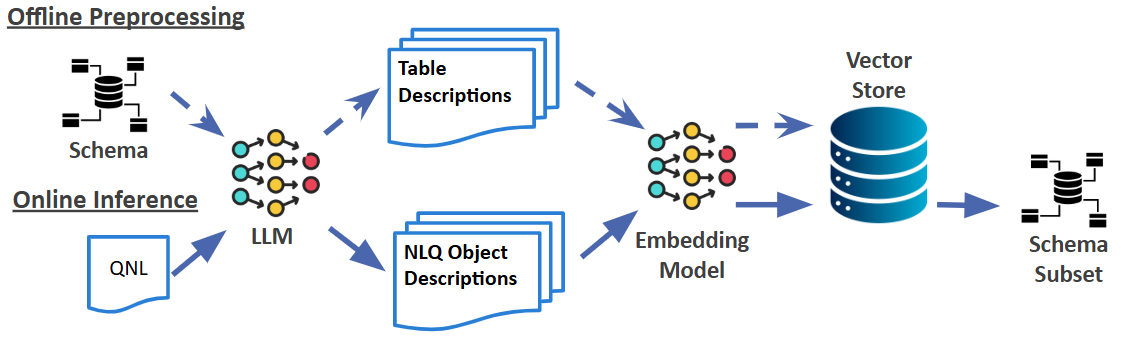
\includegraphics[width=\linewidth]{figures/skalpel-diagram.png}
  \caption{The prototype \PROJECTNAME{ }subsetter combines LLM-based question decomposition and embedding vector generation to perform table retrieval from a vector store. \PROJECTNAME{ } measures cosine distance between the embeddings of 2-3 sentence table descriptions and a set of object descriptions decomposed from an NLQ and returns tables and all of their columns whose distance are below a set threshold.}
  \label{fig:skalpelarchitecture}
\end{figure}

In addition to a thorough evaluation of existing subsetting modules, we capitalize on our analysis to prototype a subsetting method targeted at improving NL-to-SQL for very large database schemas (Figure~\ref{fig:skalpelarchitecture}).
The primary design goal of \PROJECTNAME{ }is to maximize table and column recall while minimizing subset size without compromising recall, minimizing token usage, and reducing latency.

To accomplish this goal, we adopt a hybrid approach similar to Crush4SQL~\cite{kothyari-etal-2023-crush4sql} except instead of schema hallucination, we task the LLM to decompose the question (similarly to the decomposition method described in ~\cite{Katsogiannis-Meimarakis2026}) with the instruction ``describe the various objects, concepts, etc. in a natural language query.''
The output of the object description task is embedded using the NovaSearch \emph{stella\_en\_1.5B\_v5} embedding generation model~\cite{zhang2025jasperstelladistillationsota}.

During an offline preprocessing stage, \PROJECTNAME{ }uses an LLM to generate natural language descriptions of schema tables using the table name, column names, and example values.
These descriptions are also embedded using NovaSearch and stored in a PGVector~\cite{pgvectorrepo} database.
During subset generation, \PROJECTNAME{ }retrieves relevant tables and all their columns via cosine distance search, retrieving all tables where the distance between question decomposition embeddings and table description embeddings are less than or equal to 0.525.


\section{Schema Subsetting}


Schema knowledge subsetting (also known as schema linking) is the process of extracting a subset of relations and attributes from a database schema with the objective of eliminating as many unneeded identifiers while retaining all identifiers required for a correct query generation.

In this section, we review recent subsetting modules in NL-to-SQL systems ranked highly on the Bird benchmark, we measure subsetting effectiveness by ablating schema knowledge representations from a full schema to only identifiers present in a correct query, we establish symbolic definitions of the subsetting problem, and articulate some challenges relating to mismatches between natural language questions and schema identifiers. 

\subsection{Survey of Subsetting Approaches}

Many leading submissions to the Bird NL-to-SQL benchmark~\cite{benchmark-bird}, including the top performer, use schema subsetting.
As of June 2025, 5 out of the top 15 entries~\cite{shkapenyuk2025automaticmetadataextractiontexttosql,gao2025previewxiyansqlmultigeneratorensemble, xie2025opensearchsqlenhancingtexttosqldynamic, donder2025cheaperbetterfasterstronger,talaei2024chesscontextualharnessingefficient} on Bird's execution accuracy leaderboard use some form of schema subsetting in their SQL generation pipelines.
While some analysis suggests that the risk of omitting required identifiers during the subsetting step negates any potential benefit~\cite{maamari2024deathschemalinkingtexttosql}, the overall performance of the top submissions that use schema subsetting suggest that, when done correctly, subsetting may be improving NL-to-SQL performance in some cases.
These mixed results motivate additional scrutiny of existing schema subsetting methods to 1) determine their overall usefulness for improving NL-to-SQL, and 2) discover specific aspects of subsetting methods that either improve or degrade NL-to-SQL generation.

\begin{figure}
  \centering
  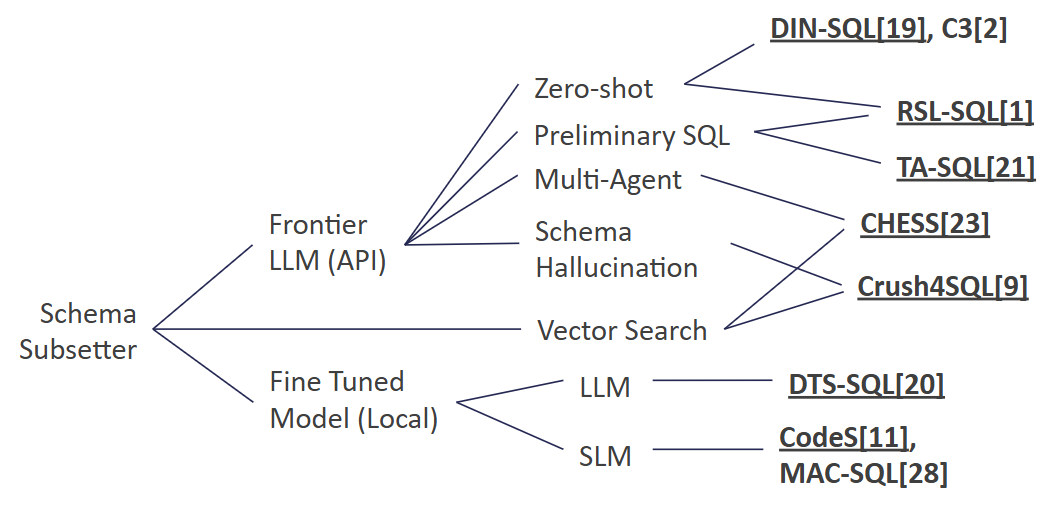
\includegraphics[width=\linewidth]{figures/subsetter-taxonomy.png}
  \caption{Schema subsetting methods use a variety of techniques and resources including frontier (API-based) LLMs, smaller locally-hosted and finetuned models (both LLM and SLM), and vector search. Some methods use more than one method such as CHESS which uses multiple LLM agents and vector search. Underlined methods indicate that a method is included in our experiments.}
  \label{fig:subsetting-taxonomy}
\end{figure}

\paragraph{\textbf{Selection Criteria for Evalution}}

Our research objective is to evaluate the best representations of a variety of subsetting methods, most of whose relatively high positions on the Bird execution accuracy leaderboard indicates good performance.
Our ability to reproduce a given subsetting method is limited by code and model availability, and this constraint eliminates a large proportion of entries, as only 34 of the 74 entries provide links to their source code.
Of the remaining entries, we select entries that indicate the use of a schema subsetting step and provide a fully reproducible codebase and, where applicable, model weights.
Figure ~\ref{fig:subsetting-taxonomy} shows the 7 subsetting methods we evaluate in our research and their classification in terms of subsetting model type and technique.

\paragraph{\textbf{Subsetting with LLMs}} 
Several approaches make use of the same LLM used for NL-to-SQL generation in a prior step that includes submitting a full schema, a natural language question, and instructions to identify the most-relevant schema entities.
The output of this reduction step is typically used as input to an SQL generation prompt.
LLM-based subsetters are subject to the same context limit constraints as an SQL generation prompt, and so a database schema representation that is too large for naive NL-to-SQL inference with full schema knowledge will also be too large for a schema subsetting prompt.

DIN-SQL~\cite{pourreza2023dinsql}, and C3~\cite{dong2023c3} use LLM-based schema subsetters as preliminary actions in a multi-step zero-shot NL-to-SQL generation pipelines.
RSL-SQL~\cite{cao2024rslsqlrobustschemalinking} uses an LLM-based bi-directional subsetting method that combines the results of two actions: 1) a few shot prompt instructing the LLM to select relevant schema elements based on a natural language question, and 2) and extraction of table and column names from a \emph{preliminary SQL} query generated via zero-shot prompting and the full schema representation. 
TA-SQL~\cite{qu2024generationalignitnovel} pre-processes a database with LLM-generated column descriptions which are used to supplement schema knowledge representations in a zero-shot SQL generation prompt.
TA-SQL generates subsets through identifier extraction from the generated preliminary SQL queries.

\paragraph{\textbf{Hybrid Subsetting Methods}}

Some methods employ multiple techniques including the use of both LLMs and semantic search.
CHESS~\cite{talaei2024chesscontextualharnessingefficient} is an agentic system that contains information retriever and schema selector agents that execute their tasks sequentially to generate schema subsets. 
The information retriever agent has access to information retrieval tools that use vector searches over identifier embeddings to retrieve the most relevant identifiers.
The schema selector agent refines the information retriever's selections using LLM-based few shot prompting.
Crush~\cite{kothyari-etal-2023-crush4sql} is the only method that does not correspond to a Bird benchmark entry. It is an LLM-based subsetter that introduces the novel idea of schema hallucination as a pre-step to semantic search of vector representations of the target database's identifiers.

\paragraph{\textbf{Subsetting with Finetuned Models}}

Another approach is to finetune a smaller language model (SLM) specifically to the task of schema subsetting.
DTS-SQL~\cite{pourreza2024dtssql} uses a finetuned 7B parameter Deepseek Coder~\cite{deepseek-coder} to subset schemas by selecting relevant tables. 
Code-S~\cite{li2024codes} employs a pre-trained T5-based model and adds a value lookup feature that seeks alignment between natural language symbols and text values in a target database. Code-S employs subsetting-specific analysis via area under curve (AUC) metrics for table and column recall.
The authors of DTS-SQL introduce the use of precision and recall to evaluate schema linking performance separately from overall NL-to-SQL performance.
MAC-SQL~\cite{wang2024macsql} uses a selector agent composed of an LLM prompt sequence run against a finetuned 7B parameter LLM to reduce a database to a subset database aligned with an input natural language question. 



\subsection{Subsetting Effectiveness}

\paragraph{\textbf{Schema Subset Proportion Effects on NL-to-SQL}}

\begin{figure}
  \centering
  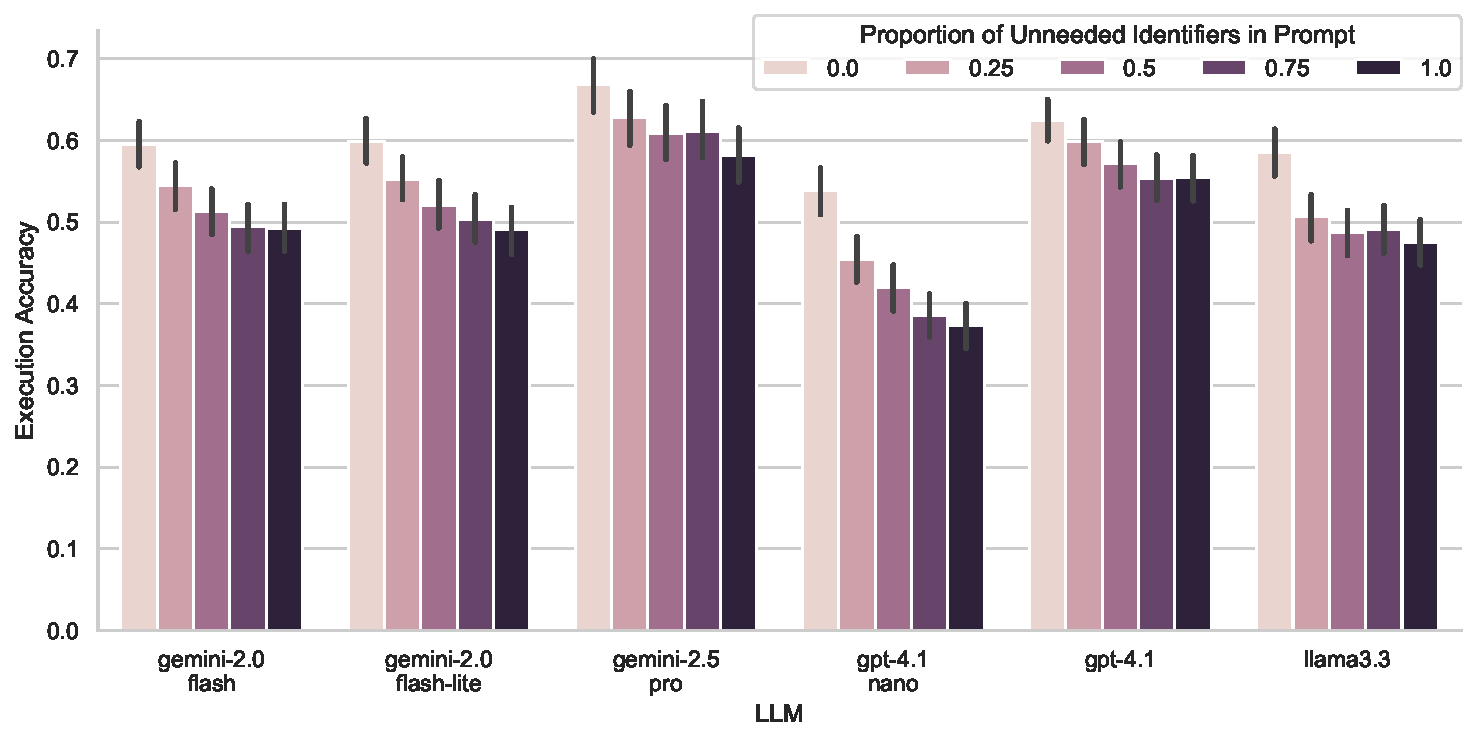
\includegraphics[width=\linewidth]{./figures/execution_accuracy_by_identifier_proportion_barplot.pdf}
  \caption{Execution accuracy (y-axis) over the medium- and large-sized schemas in the Snails benchmark generally exhibits a downward trend as the proportion of unneeded identifiers increases.}
  \label{fig:schema-reduction-graph}
\end{figure}

To test the assumption that schema subsetting improves NL-to-SQL performance, we perform subset proportion ablation where we modify schema representations iteratively to randomly reduce the proportion of unneeded schema identifiers in a SQL creation prompt, where a proportion of 1.0 contains all schema identifiers, and a proportion of 0.0 contains only the identifiers required for a correct result.
Figure \ref{fig:schema-reduction-graph} shows the result of a zero-shot prompt with varying proportions of schema knowledge executed over the SNAILS benchmark dataset at the Native naturalness level.
Except for GPT-4.1 Nano, there is no improvement at the 0.75 proportion mark, and only the GPT 4 model family exhibits improvement at 0.50. All models show consistent improvement when the schema representation is further reduced to 0.25. 
When the schema representation sheds all unneeded identifiers (the case of a perfect subset), execution accuracy improves dramatically for all models.
Logistic regression confirms a significant negative effect of more unneeded identifiers, with accuracy declining as unneeded identifier proportions increase (p < 0.0001).
The relatively low $R^2$ values between 0.01 and 0.025 (model-dependent) suggest that additional factors besides schema proportion also affect execution accuracy.

The takeaway from this evaluation is twofold: 1) the usefulness of schema subsetting at different proportions is model-dependent, and 2) the potential for performance improvement in the case of a subset with perfect recall motivates further evaluation and improvement of real-world subsetting methods.

\subsection{Definitions}

\paragraph{\textbf{Schema and Database}}

We evaluate subsetting processes over a relational database schema $\SCHEMA$ that contains a set of relations $\RELATIONS$ and their attributes $\ATTRIBUTES \in \RELATIONS$.
Each relation $\RELATIONS$ is a bag of tuples $\TUPLE_{1...n}$ where $t[\ATTRIBUTES]$ references an atomic value $\VALUE$ of the type of attribute $\ATTRIBUTES$. 
The database instance $\DATABASE$ is the realization of $\SCHEMA$ such that 
$t[\ATTRIBUTES_{1...n}] \in \RELATIONS_{1...n} \in \SCHEMA \Rightarrow \DATABASE$, and an SQL query $\SQLQUERY$ over $\DATABASE$ returns a result $\RESULT$ which is also a bag of tuples.
We denote the set of all values $\VALUE$ in $\DATABASE$ as $\VALUES$, and specify the set of all values in a given relation or a relation and attribute as $\VALUES_\RELATIONS$ and $\VALUES_{\RELATIONS.\ATTRIBUTES}$ respectively.

\paragraph{\textbf{SQL Queries and Identifiers}}
An SQL query $\SQLQUERY$ references relations $\RELATIONS$ and attributes $\ATTRIBUTES$ in its projection and selection clauses. 
We differentiate between SQL queries that are members of benchmark question and query pairs as ``gold'' queries, with the notation $\SQLGOLD$ and queries that are predicted by an NL-to-SQL function with the notation $\SQLPRED$.
For the purposes of subsetting analysis, we consider $\SQLQUERY$ in a syntax-agnostic manner, simply as a set of its identifiers organized as a schema subset $\SUBSET$ containing a subset of schema relations $\RELATIONS'$ and attributes $\ATTRIBUTES'$.

% $\mathbf{I}^{sql}$ which can be either relations $\mathbf{I}_{\RELATIONS}^{sql}$ or attributes $\mathbf{I}_{\ATTRIBUTES}^{sql}$.

We also define selection clause predicates $\PREDICATES$ in simple terms of an attribute $\ATTRIBUTES$ and value $\VALUE$, and denote them in the form $\PREDICATES := <\ATTRIBUTES, \VALUE>$ where for a given predicate $\PREDICATES$, $\PREDICATES_\ATTRIBUTES$ and $\PREDICATES_\VALUE$ are the attribute and value referenced in the clause.
For example,\\ $\PREDICATES := <customer.name, jones>$ represents the selection expression $customer.name = ``jones"$.

\paragraph{\textbf{Benchmarks and Natural Language Question Symbols}}
A natural language question $\QNL$ is comprised of symbols $\NLSYMBOL \in \QNL$ where symbols may be words, numbers, or special characters. 
$\QNL$ is an ordered concatenation of $\NLSYMBOL_{1...n}$ whereas the unordered set of $\NLSYMBOL \in \QNL$ is denoted as $\WORDSNL$. 
The distinction between $\QNL$ as ordered, and $\WORDSNL$ as unordered is a necessary distinction in some contexts defined in subsequent sections.

Nl-to-SQL benchmarks $\BENCHMARK$ are collections of databases $\DATABASE$ and associated natural language question $\QNL$ and gold SQL query $\SQLGOLD$ pairs.
We denote each pair of $\QNL, \SQLGOLD \in \DATABASE \in \BENCHMARK$ as $\QUESTIONPAIR$ so that $\QUESTIONPAIR := <\QNL, \SQLGOLD>$.

\paragraph{\textbf{Subsetting Function}}
We define an abstract schema subsetting function $\SUBSETFUNCTION$ which generates a schema subset $\SUBSET$ given the inputs $\QNL$ and $\DATABASE$. 
This function uses an abstract comparison operation denoted as $\SIMILAR$ (and its negation $\NOTSIMILAR$) which is satisfied if there is sufficient semantic similarity or other relevance-defining relationship between one or more symbols in $\QNL$ and one or more entities in a database $\DATABASE$.

$$\SUBSETFUNCTION(\QNL, \DATABASE) \rightarrow \{\SUBSET | \SUBSET\subseteq \SCHEMA\}$$

where relations and attributes are included in the subset by the criteria:
\begin{multline}
\SUBSETFUNCTION(\QNL, \DATABASE) := \forall \NLSYMBOL \in \QNL \exists \RELATIONS | \RELATIONS \in \DATABASE \land \\
(\RELATIONS \SIMILAR \NLSYMBOL \lor (\exists \ATTRIBUTES \in \RELATIONS | \ATTRIBUTES \SIMILAR \NLSYMBOL))
\end{multline}
That is, relations and attributes are members of the schema subset $\SUBSET$ if they satisfy the semantic similarity comparison operation $\SIMILAR$ for at least one symbol $\NLSYMBOL$ in $\QNL$.
Note that there is no restriction on the $\SIMILAR \QNL$ operation so that we can overload $\SUBSETFUNCTION $ and its $\SIMILAR$ operator in specific implementations in subsequent sections.



\subsection{Subsetting Challenges}
\label{sec:subsetting-challenges}

The schema subsetting process presents several challenges including relation and attribute name ambiguities, unmentioned attributes required for correct SQL statements, and unnatural schema elements with minimal association with common natural language terms.
In this section, we formalize two such problems relating to recall errors caused by mismatches between natural language questions and their associated gold queries.

\paragraph{\textbf{The Value Reference Problem}}
$\QNL$ references an instantiation of an object (e.g., proper nouns such as names and places) but not the type of object.
For example, the question \emph{how many Toyota Tacomas were involved in rollover accidents in 2022?} requires the retrieval of the Make and Model columns within a vehicle information table.
However, the question does not contain keywords that will match \emph{Toyota} or \emph{Tacoma} to either the Make or Model attributes.
We refer to this problem as the \textbf{\emph{value reference}} problem.
We can identify occurrences of the value reference problem by the criteria:

\begin{equation}
  \forall \PREDICATES \in \SQLQUERY \exists \NLSYMBOL \in \WORDSNL | \NLSYMBOL \SIMILAR \PREDICATES_v \land \NLSYMBOL \NOTSIMILAR \PREDICATES_\ATTRIBUTES
\end{equation}

That is, there is a satisfied similarity between a symbol in $\QNL$ and at least one value in any predicate $\PREDICATES$ in $\SQLQUERY$, where the symbol does not also satisfy a similarity comparison with at least 1 attribute or relation identifier in the same $\SQLQUERY$.

Value lookup is an approach used by CodeS~\cite{li2024codes} where a $\QNL \SIMILAR \VALUES$ operation extracts attributes containing values relevant to $\QNL$.
The CRUSH subsetting approach relies on LLM prompting to hallucinate a schema in reponse to a $\QNL$, which results in the generation of an intermediate representation of $\WORDSNL$ that better aligns with a value in $\VALUES$~\cite{kothyari-etal-2023-crush4sql}.

\paragraph{\textbf{The Hidden Relation Problem}}

$\QNL$ contains keywords that bear semantic similarity to relations in $\SCHEMA$, and at least one transitive dependency exists between relations that does not correspond to a $\QNL$ keyword.
We refer to this problem as the \textbf{\emph{hidden relation}} problem.
The hidden relation problem defined as:

\begin{equation}
   \forall \NLSYMBOL \in \WORDSNL \exists \RELATIONS \in \SQLQUERY | \RELATIONS \NOTSIMILAR \NLSYMBOL \land (\forall \ATTRIBUTES \in \RELATIONS| \ATTRIBUTES \NOTSIMILAR \NLSYMBOL)
\end{equation}

That is, there is at least 1 relation identifier $\RELATIONS$ in a query $\SQLQUERY$ that neither itself, nor any of its attributes $\ATTRIBUTES$, satisfies a similarity comparison with any symbol $\NLSYMBOL$ in $\WORDSNL$.
This problem typically arises when a $\SQLQUERY$ must contain intermediate joins with relations that are not semantically similar to any keywords or phrases in a natural language question.



\section{Experiments}



\subsection{Discovering Schema Size Limits}
In order to discover the limits of subsetting methods executed over large schemas, we assess subsetting method capabilities in the context of schema size categories (described in Table~\ref{tab:benchmark-schema-sizes}).
We do this by determining the percent of subsetting attempts that yield a non-empty set of schema identifiers, which indicates that the subsetting method did not encounter a condition that prevented it from generating a subset.

\paragraph{\textbf{Size Constraints}}
\begin{table}
\caption{Percent of each schema size category that each subsetting method is capable of processing. Only 3 of the 7 evaluated methods are capable of processing all schemas.}
\label{tab:schema-size-limits}
\begin{tabular}{llllll}
\toprule
$\Psi$ & S & M & L & XL & XXL \\
\midrule
CodeS & 100\% & 100\% & 100\% & 100\% & 100\% \\
DINSQL & 100\% & 100\% & 100\% & 100\% & 100\% \\
chess & 100\% & 100\% & 100\% & - & - \\
crush4sql & 100\% & 100\% & 100\% & 100\% & 100\% \\
dtssql & 66\% & 12\% & - & - & - \\
rslsql & 100\% & 100\% & 82\% & 79\% & - \\
skalpel & 100\% & 100\% & 100\% & 100\% & 100\% \\
tasql & 100\% & 100\% & 100\% & 86\% & - \\
\bottomrule
\end{tabular}
\end{table}

Exposing subsetting methods built to solve smaller schemas in the Bird benchmark to larger schemas in the Snails and Spider 2 benchmarks reveals some limitations in most of the subsetting methods.
Methods that load the entire schema representation into a single LLM prompt tend to exceed LLM context window limitations on very large schemas. 
Only 3 of the 7 methods that we evaluate successfully completing inference over all benchmark schemas. 
Table~\ref{tab:schema-size-limits} reveals the inference completion percentages for each model and schema size.
CodeS, a machine-learning based classifier approach, handles its small 512 token context via partitioning. 
Crush4SQL is not subject to context window constraints because it performs table and column retrieval using semantic search.
DINSQL generates a minimal schema representation without additional value examples or identifier descriptions and thus does not exceed the GPT4.1 context window.
Chess did not exceed any context limitations, however it relies on a column-by-column assessment to determine column relevance--a method that proves to be prohibitively expensive and time consuming for very large schemas.
In the following experiments, we only compare results for subsetting attempts that do not exceed a subsetting method's capabilities.

\subsection{Experiment 1: Subsetting Performance}
\label{subsection:experiment1}

We evaluate 7 subsetting methods used by high-performing NL-to-SQL submissions on the Bird~\cite{benchmark-bird} benchmark leaderboard.
These methods represent a variety of approaches including frontier LLM prompting, SLM finetuning, and semantic search.
We go beyond the standard measures of precision, recall, f1, and also include token usage (as applicable), inference time, preprocessing time (as applicable), and subset size as a proportion of the full schema.
This allows us to assess the time and resource requirements for each subsetting method, and motivates the development of more economical methods.

\paragraph{\textbf{Research Question}} What are the best--measured in terms of recall, precision, f1, time-based performance, and resource usage--methods for correctly reducing the size of LLM prompt schema knowledge representations? 

\paragraph{\textbf{Evaluation Method}}
We evalute subsetting performance over the NL-SQL question-query pairs $\QUESTIONPAIR \in \BENCHMARK$ in the Bird, Snails, and Spider 2 benchmarks.
The correct subsets used to derive recall, precision, and f1 scores include all identifiers (relations and attributes) present in each pair's gold SQL representation $\SQLGOLD$.

In order to derive the correct subset for each benchmark question, we define an SQL parsing function $P(\SQLQUERY) \rightarrow \SUBSET$ that arranges relations and attributes into a schema subset $\SUBSET$ comprised of identifiers referenced in the input query $\SQLQUERY$.
For each $\QUESTIONPAIR$ in a benchmark $\BENCHMARK$, we derive a gold scema subset $\SUBSETGOLD$ using $P(\SQLGOLD) \rightarrow \SUBSETGOLD$.
Because $\SQLGOLD$ is a syntactically correct query over its target $\DATABASE \in \BENCHMARK$, we assert that all $\SUBSETGOLD \subseteq \SCHEMA$ and that $\SUBSETGOLD$ represents the execution of a perfect (or oracle) subsetter $\SUBSETFUNCTION(\QNL, \DATABASE) \rightarrow \SUBSET$.
With this assertion, we evaluate the output $\SUBSETPRED$ of each subsetting method's implementation of $\SUBSETFUNCTION$ against $\SUBSETGOLD$ for each $\QUESTIONPAIR$.

\begin{multline}
  \forall \QNL, \SQLGOLD \in \QUESTIONPAIR \in \mathbf{B}: 
  \\ \SUBSETFUNCTION(\QNL, \DATABASE) \rightarrow \SUBSET_{pred}; P(\SQLGOLD) \rightarrow \SUBSETGOLD
\end{multline}

The end state of the process is a collection of predicted and gold subsets for all question-query pairs used as the input to the analysis described in the following sections. 

\paragraph{\textbf{Evaluation Metrics}}

Schema linking-specific metrics have begun to appear in recent NL-to-SQL papers including precision and recall~\cite{pourreza2024dtssql, kothyari-etal-2023-crush4sql,benchmark-snails, Katsogiannis-Meimarakis2026, maamari2024deathschemalinkingtexttosql}, and AUC~\cite{li2024codes}.
To the best of our knowledge, our work is the first application of schema linking metrics to a comparison of multiple reproductions of schema linking modules used in real-world NL-to-SQL systems.
Additionally, we believe this to be the first work to evaluate schema subsetting in terms of efficiency by measuring token usage, offline pre-processing time, and inference time.

We evaluate performance of $\SUBSETFUNCTION$ using the following metrics.
\begin{itemize}
  \item SchRecall: $|\SUBSETGOLD \cap \SUBSETPRED| / |\SUBSETGOLD|$
  \item PerfRecall: 1 if \emph{ScheRecall} = 1.0, 0 otherwise
  \item SchPrecision: $|\SUBSETGOLD \cap \SUBSETPRED| / |\SUBSETPRED|$
  \item SchF1: $2 * (SchRecall * SchPrecision) / (SchRecall + SchPrecision)$
  \item Subset Proportion: $|\SUBSETPRED| / |\SCHEMA|$; (lower is better)
  \item Inference Time: Time (in sec.ms) to execute $\SUBSETFUNCTION$
  \item Prompt Token Count (LLM-based): Sum of LLM tokens used by $\SUBSETFUNCTION$ to generate $\SUBSETPRED$
  \item Preprocessing Rate: $SchemaProcessingTime / |\ATTRIBUTES \in \SCHEMA|$ where \emph{SchemaProcessing} is the time in seconds required to perform pre-processing tasks such as generating vector embeddings or data descriptions.
\end{itemize}
We expand the evaluation framework further by generating each of the listed metrics for each identifier type (relations and attributes).
\begin{itemize}
  \item SchRelRecall: $|\RELATIONSSUBSETGOLD \cap \RELATIONSSUBSETPRED| / |\RELATIONSSUBSETGOLD|$
  \item SchRelPrecision: $|\RELATIONSSUBSETGOLD \cap \RELATIONSSUBSETPRED| / |\RELATIONSSUBSETPRED|$
  \item SchRelF1: $2 * (SchRelRecall * SchRelPrecision) / \\ (SchRelRecall + SchRelPrecision)$
  \item Relation Proportion: $|\RELATIONSSUBSETPRED| / |\RELATIONS \in \SCHEMA|$; (lower is better)
  \item SchAtrRecall: $|\ATTRIBUTESSUBSETGOLD \cap \ATTRIBUTESSUBSETPRED| / |\ATTRIBUTESSUBSETGOLD|$
  \item SchAtrPrecision: $|\ATTRIBUTESSUBSETGOLD \cap \ATTRIBUTESSUBSETPRED| / |\ATTRIBUTESSUBSETPRED|$
  \item SchAtrF1: $2 * (SchAtrRecall * SchAtrPrecision) / \\ (SchAtrRecall + SchAtrPrecision)$
  \item Attribute Proportion: $|\ATTRIBUTESSUBSETPRED| / |\ATTRIBUTES \in \SCHEMA|$; (lower is better)
\end{itemize}

\paragraph{\textbf{Performance Constraints}}
While variance in precision indicate method quality, other metrics indicate method feasibility where failure to meet specific constraints will result in NL-to-SQL translation failure.
That is not to say that a method should be discounted outright in the event of a failure to meet the constraint in some cases, rather the frequency of failures should be compared between methods with the best methods being those with the fewest failure occurrences.

\emph{Perfect recall:} Failure of the subsetting function $\SUBSETFUNCTION$ to recall all $\ATTRIBUTESSUBSETGOLD$ and $\RELATIONSSUBSETGOLD$ in $\SQLGOLD$ will almost always ensure failure in the downstream NL-to-SQL translation task.
Thus, it is imperative that we evaluate recall in the strictest terms possible with the goal of identifying methods that yield recall values as close to 1 as possible.
The proportion of subsetting attempts that achieve perfect recall over all attempts represents the likely upper bound of execution accuracy in a subsequent NL-to-SQL step.
Subsetting methods that achieve perfect recall scores below downstream NL-to-SQL (sans subsetting) execution accuracy proportion scores are likely to reduce overall performance.  

\emph{Subset size:} schema subsets must be sufficiently small that generated prompts fit within the target LLM's context window token limitations.
Subsetting attempts that fail due to context window constraints are omitted from analysis.
Subsetting method schema coverage (the percentage of schemas each method is capable of handling) is measured in Table~\ref{tab:schema-size-limits}, and represented as a proportion in Figure~\ref{fig:subsetting-performance_radar}.

\paragraph{\textbf{Subsetting Challenges Analysis}}
We apply the subsetting challenge definitions in Section \ref{sec:subsetting-challenges} to categorize failures and isolate failure causes.
Identifying subsetting challenge-related failure states requires an implementation of the semantic similarity comparison operation denoted as $\SIMILAR$. 
We make use of the NovaSearch \emph{stella\_en\_1.5B\_v5} embedding generation model~\cite{zhang2025jasperstelladistillationsota} with a sequence length of 1,024 and store the embeddings in a PGVector database. 
The similarity comparison operation $\SIMILAR$ is satisfied when the cosine distance between two sequences is below a similarity distance threshold. 
We derive the similarity threshold through iterative evaluation of threshold values, selecting the value that yields the most satisfactory results as determined by a human researcher.


\subsection{Experiment 2: NL-to-SQL Performance}

Because the objective of schema subsetting is improving NL-to-SQL performance, the most important measure of a subsetting method is to evaluate its effect on NL-to-SQL performance.
To this end, we ask the following research questions:

\paragraph{\textbf{Research Question 1}} To what extent (if any) do schema subsetting methods improve NL-to-SQL execution accuracy?

\paragraph{\textbf{Research Question 2}} To what extent (if any) does the size of a schema affect the usefulness of schema subsetting? 

\paragraph{\textbf{Evaluation Method}}
The subsets $\SUBSETPRED$ generated in experiment 1 are the input to the NL-to-SQL generation in experiment 2.
We evaluate the performance of $\SQLPRED$ generated using prompts containing $\SUBSETPRED$ from all subsetting functions $\SUBSETFUNCTION$ and measure them in terms of execution accuracy to determine the effect of schema subsetting outputs on the objective NL-to-SQL process.

\paragraph{\textbf{Evaluation Metrics}} 

We evaluate NL-to-SQL in terms of execution result set matching, typically referred to as \emph{execution accuracy}.
Execution accuracy is the comparison of the results $\RESULTGOLD$ returned from a $\SQLGOLD$ query over $\DATABASE$ and $\RESULTPRED$ returned from a $\SQLPRED$ query over $\DATABASE$.
We adopt a subset-set comparison approach that accounts for the possibility that predicted queries may contain additional attributes not required in the gold query, but to not render the predicted query incorrect.
\begin{equation}
  \forall \ATTRIBUTES_{gold} \in \RESULTGOLD \exists \ATTRIBUTES_{pred} \in \RESULTPRED: (\VALUES \in \ATTRIBUTES_{gold}) = (\VALUES \in \ATTRIBUTES_{pred})
\end{equation}
That is, every attribute in the gold query must be present in the predicted query, and the values in each attribute of the predicted query must equal their corresponding attribute values in the gold query.

% We measure schema linking evaluation for NL-to-SQL using recall as the primary metric.
% We favor recall in this case to avoid penalizing the predicted query based on the presence of additional attribute projections.
% With $P(\SQLGOLD) \rightarrow I^{gold}$ and $P(\SQLPRED) \rightarrow I^{pred}$:

% \begin{itemize}
%   \item QryRecall: $|\mathbf{I}^{gold} \cap \mathbf{I}^{pred}| / |\mathbf{I}^{gold}|$
%   \item QryPrecision: $|\mathbf{I}^{gold} \cap \mathbf{I}^{pred}| / |\mathbf{I}^{pred}|$
%   \item QryF1: $2 * (QryRecall * QryPrecision) / (QryRecall + QryPrecision)$
% \end{itemize}

% We measure token efficiency using a tokenizing function $\mathbf{T}$ that corresponds to an LLM used to predict $\SQLPRED$ where $\mathbf{T}(prompt) \rightarrow TokenCount$ and $prompt$ is a concatenation of NL-to-SQL instructions, the schema subset extraction of $\SUBSETFUNCTION(\QUESTIONPAIR_{nl}, \DATABASE)$, and $\QNL$. 

% \paragraph{Performance Constraints} We impose the additional constraint of prompt token count to verify that the $prompt$ object token count falls within the limits of an LLM's context window.


\section{Results}


\subsection{Experiment 1: Subsetting Performance}

\begin{figure*}
  \centering
  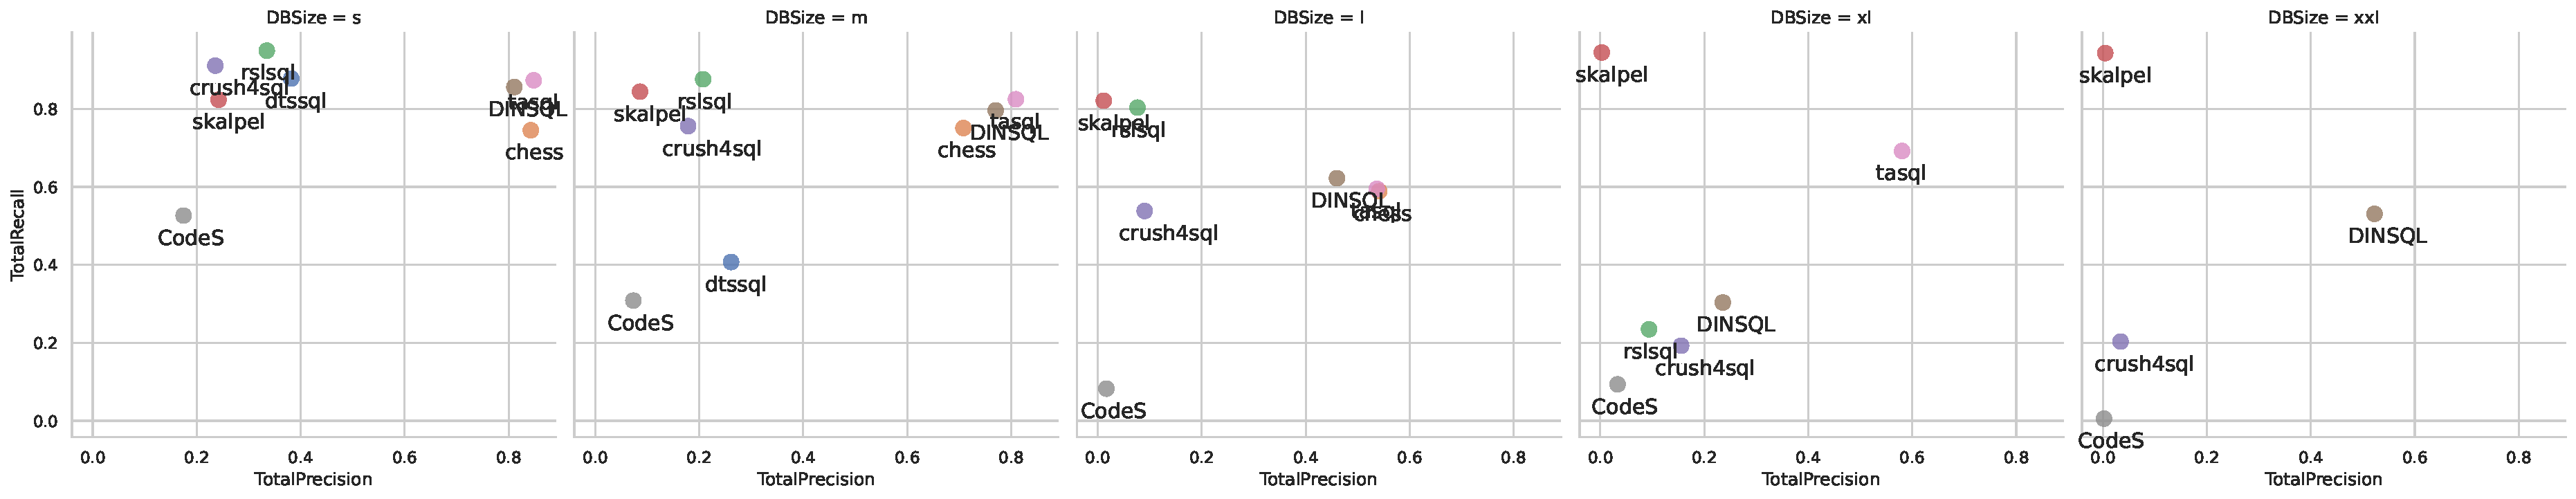
\includegraphics[width=\linewidth]{figures/pareto_total_recall_precision_by_dbsize.pdf}
  \caption{Mean total precision (x-axis) and mean total recall (y-axis) for each subsetting method for each database size. Besides the obvious drop in performance as database size increases, the data hint at some Pareto-like tradeoffs between recall and precision for most subsetting methods.}
  \label{fig:pareto-total-recall-precision-by-dbsize}
\end{figure*}

\begin{figure}
  \centering
  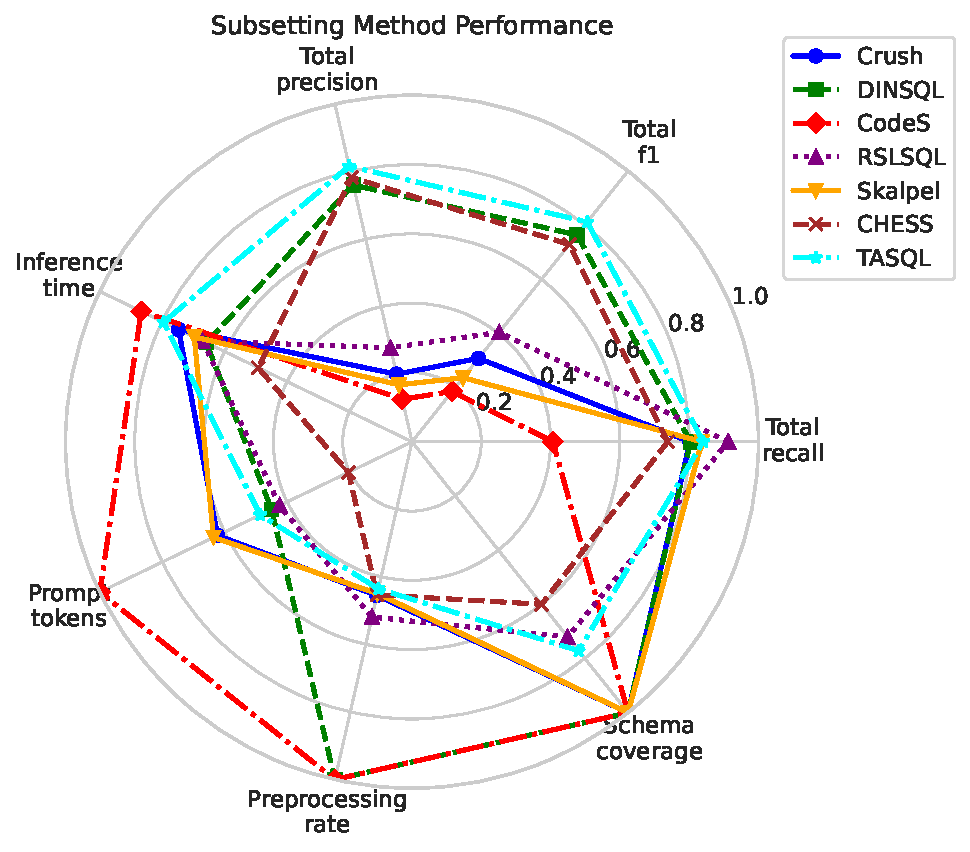
\includegraphics[width=\linewidth]{figures/subsetting_method_performance_radar.pdf}
  \caption{Inference time and Prompt tokens are log scale values with higher scores indicating better performance (e.g., lower token counts and inference time). Schema coverage indicates the proportion of the schemas in the combined benchmarks that the subsetting method can process.}
  \label{fig:subsetting-performance_radar}
\end{figure}

\paragraph{\textbf{Overall Performance}}
Overall, there is no ``best-performing method'' across all metrics and schema sizes.
Instead, we see varying performance over different schema sizes and subsetting methods that suggest the existence of Pareto-like trade spaces between various metrics (e.g., balancing precision and recall, or sacrificing latency for precision, etc.).
Also, considering that the goal of schema subsetting is to improve NL-to-SQL performance, importance must be measured against NL-to-SQL generation outcomes which we do in experiment 2.
Table~\ref{tab:exp1-all-size-schema} displays all subsetting performance metrics for each method at each schema size where only successful subsetting attempts for each method are included in the evaluation calculations.
We also display the performance differences between all methods across performance and efficiency metrics with a radar visualization in Figure~\ref{fig:subsetting-performance_radar}.

Frontier LLM-based methods including DINSQL, TASQL, CHESS, and RSLSQL generally outperform finetuned SLM- (CodeS, DTSSQL) and semantic search-based methods (Crush) by a significant margin in performance measures of f1, precision, and recall.
However, the rapid growth of token usage across schema sizes exhibited by CHESS, RSLSQL, and TASQL portray the risk of over-reliance on knowledge augmentation and granular evaluation strategies.
Knowledge enrichment, where schema representations are appended with sample values and verbose descriptions, cause both TASQL and RSLSQL to exceed 
the LLM's 1 million token context window for schemas in the XXL category.
Granular column evaluation employed by CHESS, where each column is evaluated in isolation, invokes a very high token and time cost for relatively small schemas.
The cost and time required to scale to XL and XXL schema sizes is prohibitive, and we consider it infeasible.

Recall is arguably the most important metric for evaluating the potential usefulness of a subsetting method. 
Failure to recall required identifiers all but guarantees that a subsequent NL-to-SQL translation will fail to produce a correct answer.
No method consistently produces high recall scores across all schema sizes.
Additionally, recall rates drop significantly for higher schema sizes with the ``best'' method in the XXL category only scoring an average recall of 0.53.

Setting aside the nearly terminal effect of low recall, we also want methods to reduce the schema proportion as much as possible through high precision.
TASQL's preliminary SQL parsing and identifier extraction approach yields the best schema precision in the S, M, L, and XL categories.
For the XXL category where TASQL is infeasible due to context window limitations, DINSQL achieves the highest schema precision.

Except for our own \PROJECTNAME{ }prototype subsetter, all methods reduce schema proportions below the desired target derived from our analysis of subset proportion effects on NL-to-SQL.

\begin{table*}
\caption{Experiment 1 Results: The mean of subsetting performance metrics for all $\SUBSET$ by schema size (Sz) and subsetting and subsetting 
function $\SUBSETFUNCTION$. Metrics include Inference Time (T (s)), Prompt Token Count (Tokens), Perfect Recall (PRe), 
Schema Recall (SchRe), Schema Precision (SchPr), Schema f1 (Schf1), Relation Recall (RelRe), Relation Precision (RelPr),
Relation f1 (Relf1), Attribute Recall (AtrRe), Attribute Precision (AtrPr), Attribute f1 (Atrf1), Relation Proportion (RelPn), 
and Attribute Proportion (AtrPn). Section~\ref{subsection:experiment1} provides definitions for each listed metric.}
\label{tab:exp1-all-size-schema}
\begin{tabular}{llllllllllllllll}
\toprule
 &  & T (s) & Tokens & PRe & SchRe & SchPr & Schf1 & RelRe & RelPr & Relf1 & AtrRe & AtrPr & Atrf1 & RelPn & AtrPn \\
Sz & $\Psi$ &  &  &  &  &  &  &  &  &  &  &  &  &  &  \\
\midrule
\multirow[t]{8}{*}{S} & CHESS & 31.85 & 229825 & 0.26 & 0.75 & 0.84 & 0.78 & 0.88 & 0.89 & 0.87 & 0.69 & 0.82 & 0.73 & 0.34 & \textbf{0.10} \\
 & CodeS & \textbf{0.27} & 0 & 0.20 & 0.53 & 0.17 & 0.25 & 0.66 & 0.33 & 0.42 & 0.47 & 0.14 & 0.21 & 0.71 & 0.42 \\
 & Crush & 3.06 & 425 & 0.64 & 0.91 & 0.24 & 0.36 & 0.98 & 0.39 & 0.53 & 0.88 & 0.20 & 0.32 & 0.83 & 0.49 \\
 & DINSQL & 5.89 & 4988 & 0.50 & 0.86 & 0.81 & 0.82 & 0.94 & 0.86 & 0.89 & 0.82 & 0.79 & 0.79 & 0.40 & 0.13 \\
 & DTSSQL & 9.42 & 3582 & 0.76 & 0.88 & 0.38 & 0.49 & 0.87 & \textbf{0.92} & 0.88 & 0.88 & 0.33 & 0.43 & \textbf{0.33} & 0.38 \\
 & RSLSQL & 4.52 & 8836 & \textbf{0.86} & \textbf{0.95} & 0.33 & 0.47 & \textbf{0.99} & 0.49 & 0.62 & \textbf{0.93} & 0.31 & 0.44 & 0.74 & 0.35 \\
 & Skalpel & 4.09 & \textbf{342} & 0.68 & 0.82 & 0.24 & 0.33 & 0.82 & 0.52 & 0.57 & 0.82 & 0.21 & 0.29 & 0.57 & 0.58 \\
 & TASQL & 1.51 & 2288 & 0.65 & 0.87 & \textbf{0.85} & \textbf{0.85} & 0.93 & 0.91 & \textbf{0.91} & 0.85 & \textbf{0.83} & \textbf{0.82} & 0.36 & 0.13 \\
\cline{1-16}
\multirow[t]{8}{*}{M} & CHESS & 96.69 & 891506 & 0.35 & 0.75 & 0.71 & 0.67 & 0.91 & 0.78 & 0.77 & 0.68 & 0.69 & 0.63 & 0.32 & 0.04 \\
 & CodeS & \textbf{1.15} & 0 & 0.08 & 0.31 & 0.07 & 0.11 & 0.42 & 0.16 & 0.22 & 0.26 & 0.06 & 0.09 & 0.49 & 0.12 \\
 & Crush & 2.60 & 431 & 0.41 & 0.76 & 0.18 & 0.28 & 0.91 & 0.39 & 0.51 & 0.69 & 0.15 & 0.23 & 0.41 & 0.13 \\
 & DINSQL & 8.17 & 5989 & 0.50 & 0.80 & 0.77 & 0.76 & 0.90 & 0.86 & 0.86 & 0.74 & 0.73 & 0.71 & 0.20 & \textbf{0.03} \\
 & DTSSQL & 8.82 & 7049 & 0.23 & 0.41 & 0.26 & 0.28 & 0.40 & 0.54 & 0.45 & 0.41 & 0.22 & 0.26 & 0.30 & 0.10 \\
 & RSLSQL & 10.08 & 65715 & \textbf{0.76} & \textbf{0.88} & 0.21 & 0.32 & \textbf{0.96} & 0.37 & 0.49 & 0.83 & 0.18 & 0.28 & 0.58 & 0.12 \\
 & Skalpel & 4.17 & \textbf{363} & 0.74 & 0.84 & 0.09 & 0.14 & 0.84 & 0.35 & 0.44 & \textbf{0.84} & 0.07 & 0.11 & 0.47 & 0.54 \\
 & TASQL & 2.76 & 9096 & 0.57 & 0.82 & \textbf{0.81} & \textbf{0.80} & 0.90 & \textbf{0.94} & \textbf{0.91} & 0.79 & \textbf{0.76} & \textbf{0.75} & \textbf{0.17} & \textbf{0.03} \\
\cline{1-16}
\multirow[t]{7}{*}{L} & CHESS & 351.95 & 5254439 & 0.31 & 0.59 & \textbf{0.54} & \textbf{0.54} & 0.74 & 0.63 & 0.66 & 0.51 & \textbf{0.49} & \textbf{0.48} & 0.05 & \textbf{0.00} \\
 & CodeS & 6.33 & 0 & 0.02 & 0.08 & 0.02 & 0.03 & 0.13 & 0.04 & 0.06 & 0.07 & 0.01 & 0.02 & 0.14 & 0.02 \\
 & Crush & \textbf{3.00} & 441 & 0.24 & 0.54 & 0.09 & 0.14 & 0.82 & 0.19 & 0.30 & 0.41 & 0.07 & 0.11 & 0.19 & 0.02 \\
 & DINSQL & 10.25 & 11566 & 0.43 & 0.62 & 0.46 & 0.50 & 0.71 & 0.54 & 0.59 & 0.56 & 0.42 & 0.45 & 0.06 & \textbf{0.00} \\
 & RSLSQL & 27.74 & 191906 & 0.70 & 0.80 & 0.08 & 0.13 & \textbf{0.93} & 0.35 & 0.40 & 0.73 & 0.05 & 0.09 & 0.51 & 0.05 \\
 & Skalpel & 4.21 & \textbf{380} & \textbf{0.80} & \textbf{0.82} & 0.01 & 0.02 & 0.82 & 0.13 & 0.18 & \textbf{0.81} & 0.01 & 0.02 & 0.44 & 0.49 \\
 & TASQL & 4.97 & 47440 & 0.32 & 0.60 & \textbf{0.54} & \textbf{0.54} & 0.74 & \textbf{0.69} & \textbf{0.70} & 0.51 & 0.47 & 0.47 & \textbf{0.04} & \textbf{0.00} \\
\cline{1-16}
\multirow[t]{6}{*}{XL} & CodeS & 80.50 & 0 & 0.00 & 0.09 & 0.03 & 0.05 & 0.21 & 0.09 & 0.11 & 0.06 & 0.02 & 0.03 & 0.13 & \textbf{0.00} \\
 & Crush & \textbf{4.12} & \textbf{489} & 0.00 & 0.19 & 0.16 & 0.13 & 0.47 & 0.22 & 0.23 & 0.12 & 0.11 & 0.09 & 0.18 & \textbf{0.00} \\
 & DINSQL & 35.68 & 82289 & 0.19 & 0.30 & 0.24 & 0.25 & 0.34 & 0.28 & 0.30 & 0.29 & 0.22 & 0.23 & \textbf{0.05} & \textbf{0.00} \\
 & RSLSQL & 39.02 & 498656 & 0.00 & 0.23 & 0.09 & 0.12 & 0.77 & 0.49 & 0.59 & 0.00 & 0.00 & 0.00 & 0.08 & \textbf{0.00} \\
 & Skalpel & 5.70 & 533 & \textbf{0.90} & \textbf{0.94} & 0.00 & 0.01 & \textbf{0.94} & 0.10 & 0.14 & \textbf{0.94} & 0.00 & 0.00 & 0.81 & 0.82 \\
 & TASQL & 14.62 & 294294 & 0.33 & 0.69 & \textbf{0.58} & \textbf{0.59} & 0.78 & \textbf{0.81} & \textbf{0.78} & 0.67 & \textbf{0.53} & \textbf{0.54} & \textbf{0.05} & \textbf{0.00} \\
\cline{1-16}
\multirow[t]{4}{*}{XXL} & CodeS & 381.43 & 0 & 0.00 & 0.01 & 0.00 & 0.00 & 0.01 & 0.00 & 0.00 & 0.00 & 0.00 & 0.00 & \textbf{0.00} & \textbf{0.00} \\
 & Crush & \textbf{4.49} & 431 & 0.03 & 0.20 & 0.03 & 0.06 & 0.36 & 0.04 & 0.07 & 0.15 & 0.03 & 0.05 & 0.01 & \textbf{0.00} \\
 & DINSQL & 20.79 & 384137 & 0.34 & 0.53 & \textbf{0.52} & \textbf{0.52} & 0.57 & \textbf{0.57} & \textbf{0.56} & 0.51 & \textbf{0.50} & \textbf{0.50} & \textbf{0.00} & \textbf{0.00} \\
 & Skalpel & 4.71 & \textbf{371} & \textbf{0.89} & \textbf{0.94} & 0.00 & 0.01 & \textbf{0.94} & 0.02 & 0.04 & \textbf{0.95} & 0.00 & 0.01 & 0.30 & 0.10 \\
\cline{1-16}
\bottomrule
\end{tabular}
\end{table*}


\paragraph{\textbf{Schema Size Effects on Performance}}

As schema column and table counts increase, all subsetting methods demonstrate a reduced performance across all performance measures which means that larger schemas lead to more expensive, more time consuming, and less useful results.
The Schf1 (Schema f1) column in Table~\ref{tab:exp1-all-size-schema} reveals a \emph{schema f1} performance reduction for each subsetting method as schema sizes increase.
Additionally, Figure~\ref{fig:method-radars-by-schema-size} radar charts portray consistent performance reduction for larger schemas across both performance and resource use metrics.

\paragraph{\textbf{Recall vs. Precision Trade-Off}}

Intuitively, the should be a trade-off between precision and recall, where subsetting methods that prioritize precision run an increased risk of false negatives and methods that prioritize recall would likely reduce precision to maximize the chance of true positives.
To test this intuition, we compare total precision and total recall for each method.
Figure~\ref{fig:pareto-total-recall-precision-by-dbsize} shows mean \emph{TotalPrecision} (x-axis) by mean \emph{TotalRecall} (y-axis) for each subsetting method and database size.
For the smallest databases, we can see a possible Pareto frontier with three subsetting methods (Crush, DTSSQL, and RSLSQL) clustered together with high recall and low precision, and three subsetting methods (DINSQL, TASQL, and CHESS) clustered together with high precision and slightly lower recall.
We also note that the CodeS method is well inside the frontier for all database sizes.

As database size increases, some methods retreat from the apparent frontier or disappear as they are unable to process larger schemas.
Additionally, methods that remain on the Pareto frontier generally exhibit decreased performance for larger schemas.



\begin{figure*}
  \centering
  \begin{subfigure}{0.235\linewidth}
    \centering
    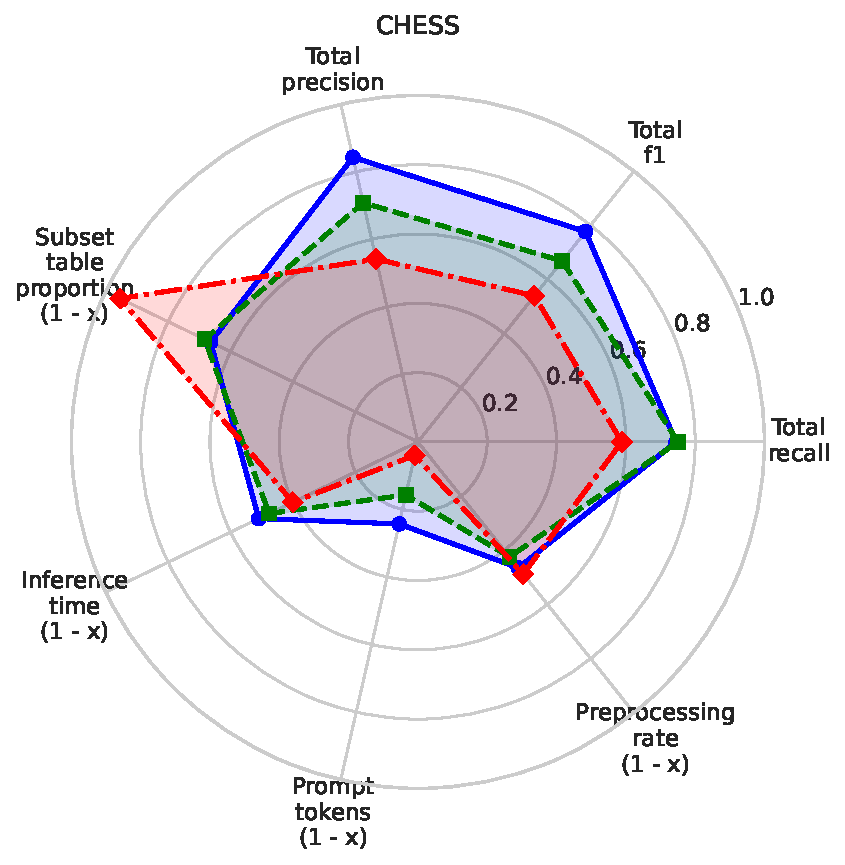
\includegraphics[width=\linewidth]{figures/method_radar_charts/chess_radar.pdf}
  \end{subfigure}
  \begin{subfigure}{0.235\linewidth}
    \centering
    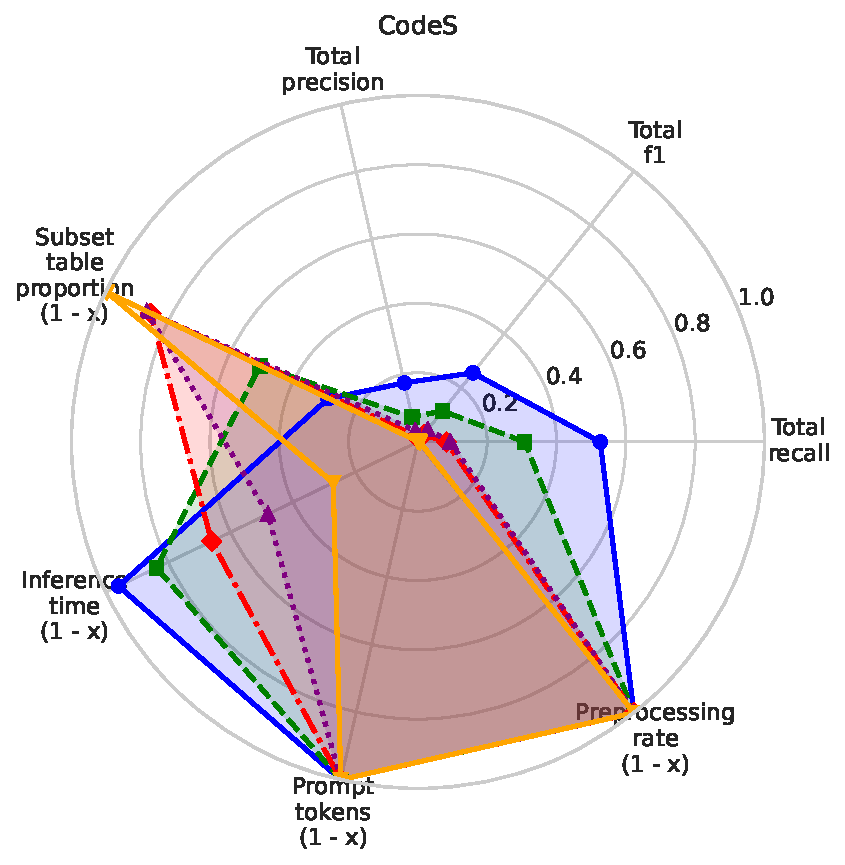
\includegraphics[width=\linewidth]{figures/method_radar_charts/CodeS_radar.pdf}
  \end{subfigure}
  \begin{subfigure}{0.235\linewidth}
    \centering
    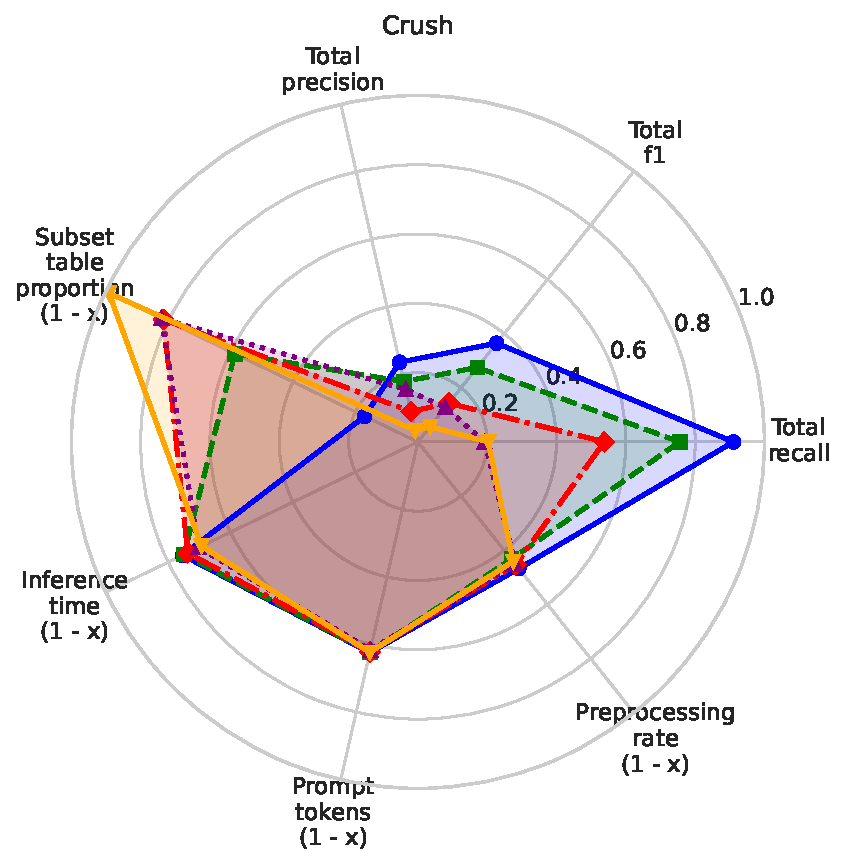
\includegraphics[width=\linewidth]{figures/method_radar_charts/crush4sql_radar.pdf}
  \end{subfigure}
  \begin{subfigure}{0.235\linewidth}
    \centering
    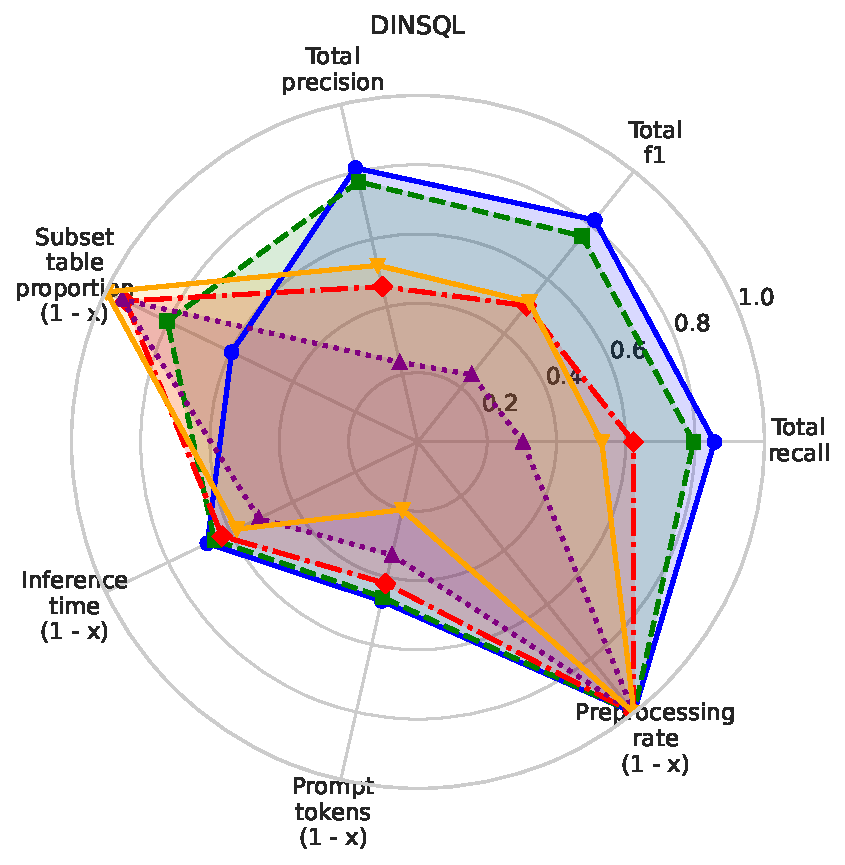
\includegraphics[width=\linewidth]{figures/method_radar_charts/DINSQL_radar.pdf}
  \end{subfigure}
  \begin{subfigure}{0.235\linewidth}
    \centering
    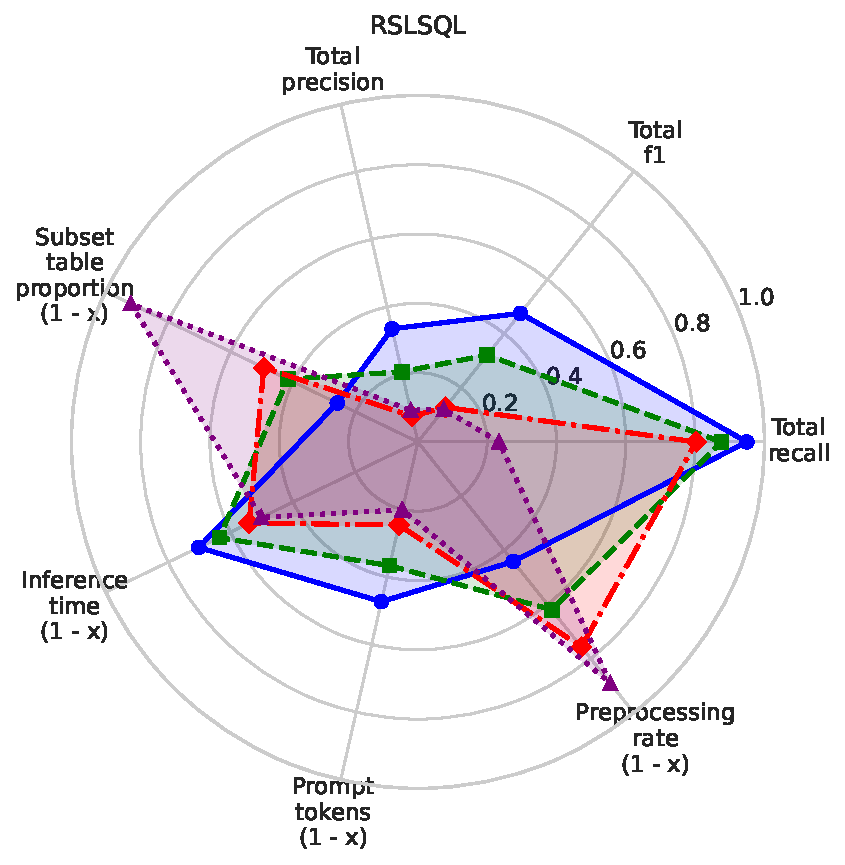
\includegraphics[width=\linewidth]{figures/method_radar_charts/rslsql_radar.pdf}
  \end{subfigure}
  \begin{subfigure}{0.235\linewidth}
    \centering
    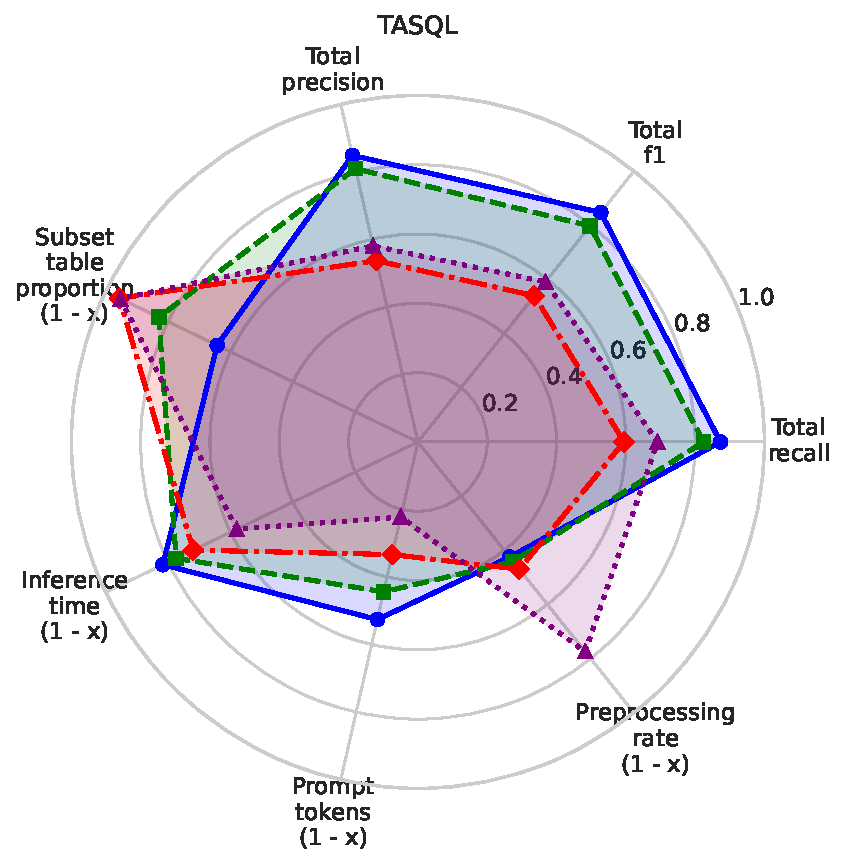
\includegraphics[width=\linewidth]{figures/method_radar_charts/tasql_radar.pdf}
  \end{subfigure}
    \begin{subfigure}{0.235\linewidth}
    \centering
    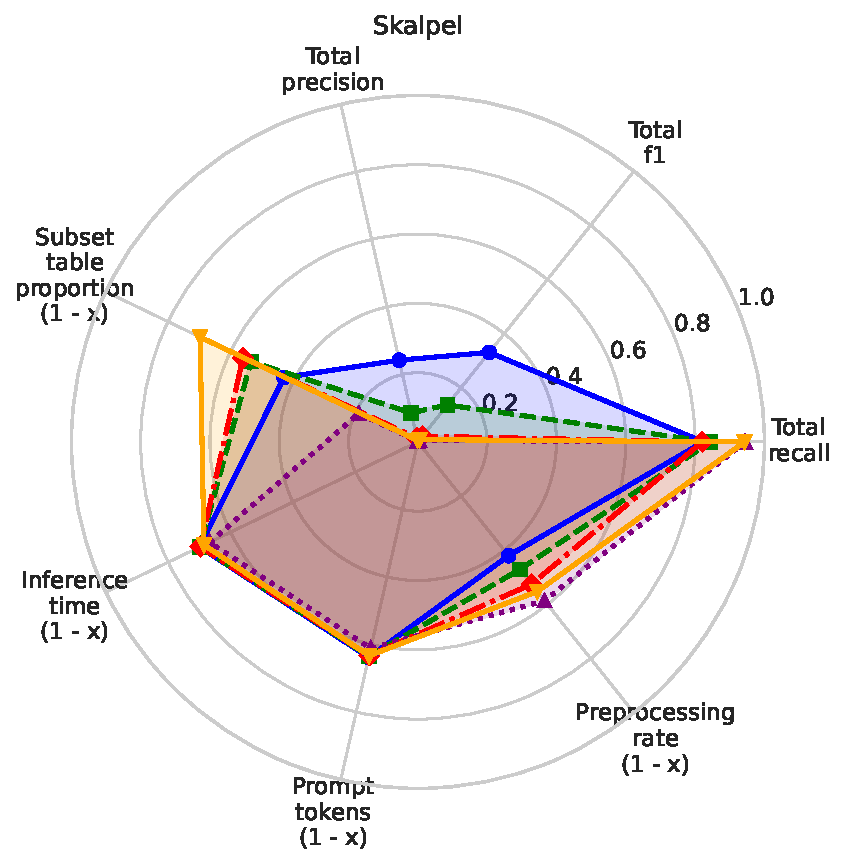
\includegraphics[width=\linewidth]{figures/method_radar_charts/skalpel_radar.pdf}
  \end{subfigure}
  \begin{subfigure}{0.27\linewidth}
    \centering
    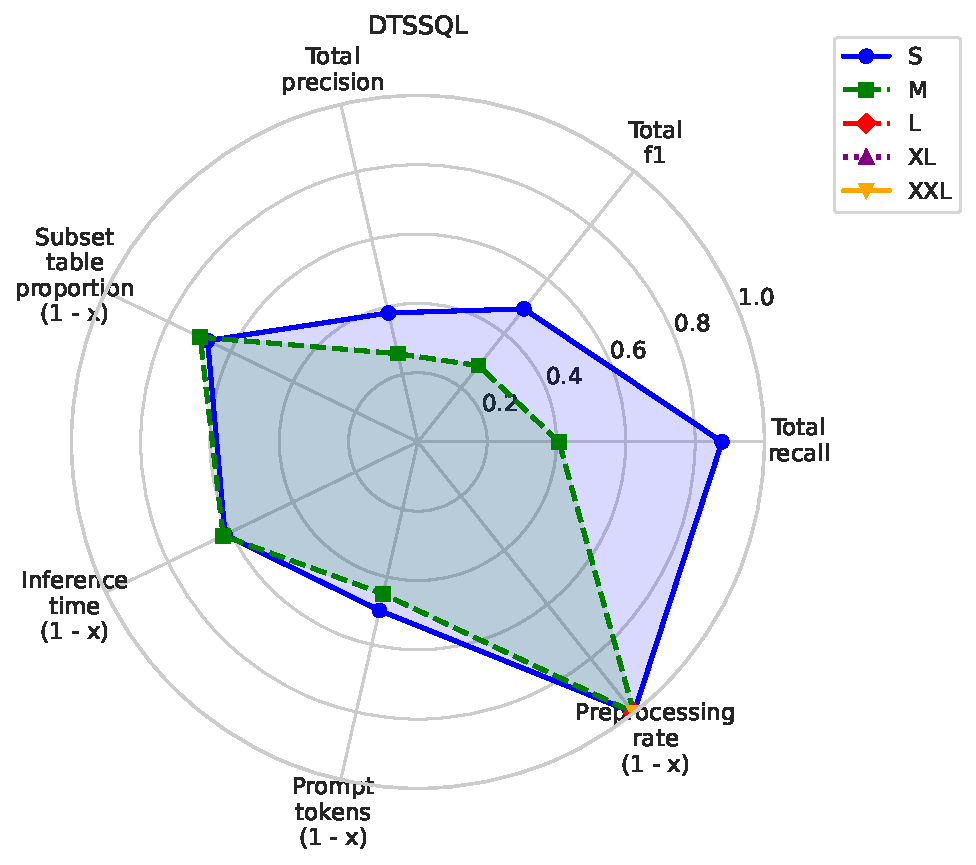
\includegraphics[width=\linewidth]{figures/method_radar_charts/dtssql_radar.pdf}
  \end{subfigure}
  \caption{These radar charts display the tradeoffs between performance (measured by precision, f1, and recall) and time and resource usage (measured by inference time, prompt tokens, and pre-processing). Sensitivity to database size (S, M, L, XL, XXL) varies by both subsetting method and measure, and generally performance across all measures decreases as database size increases. Metrics where lower is better (schema proportion, inference time, token usage, preprocessing rate) are inverted (1 - x). Inference time, prompt tokens, and preprocessing rate are fit to the range [0, 1] via natural log functions.}
  \label{fig:method-radars-by-schema-size}
\end{figure*}

\begin{table}
\caption{This table shows the Value Reference Problem (VRP) and Hidden Relation Problem (HRP) mean occurence percentages and sensitivities. Sensitivity (Sens.) is the proportion of a given problem occurence percentage (defined as realized problem over all instances where the problem might occur) to the percentage of all missing relations.}
\label{tab:vrp_hrp_sensitivity}
\begin{tabular}{lllrllr}
\toprule
$\Psi$ & \% MA & \% VRP & V-Sens. & \% MR & \% HRP & H-Sens. \\
\midrule
RSLSQL & 14\% & 7\% & 0.49 & 3\% & 11\% & 3.31 \\
DINSQL & 25\% & 17\% & 0.66 & 13\% & 22\% & 1.68 \\
TASQL & 20\% & 13\% & 0.66 & 11\% & 24\% & 2.12 \\
DTSSQL & 15\% & 11\% & 0.78 & 15\% & 29\% & 1.89 \\
CodeS & 65\% & 64\% & 0.97 & 47\% & 51\% & 1.09 \\
Crush & 32\% & 35\% & 1.11 & 11\% & 19\% & 1.71 \\
CHESS & 36\% & 43\% & 1.18 & 14\% & 31\% & 2.14 \\
Skalpel & 15\% & 21\% & 1.36 & 17\% & 58\% & 3.33 \\
\bottomrule
\end{tabular}
\end{table}


\paragraph{\textbf{Subsetting Challenges}}

To evaluate the sensitivity of subsetting methods to each subsetting challenge described in Section~\ref{sec:subsetting-challenges}, we first calculate the total percent of missing attributes and relations in $\SUBSETPRED$ from the total present in each $\SUBSETGOLD$.
Once we derive these percentages, we calculate sensitivity as the proportion of missing identifier percentages that occur when the potential for a problem manifest exists to the percentage of missing attributes in all question pairs.
Sensitivity values greater than 1 indicate that the subsetting method is more likely to omit a relation or attribute when the problem potential exists in $\QUESTIONPAIR$.

\textbf{\%MA} (missing attributes) is the mean of the percent of the count of attributes missing in $\ATTRIBUTESSUBSETPRED$ out of the total count of attributes in $\ATTRIBUTESSUBSETGOLD$ for each $\QUESTIONPAIR$. 
\textbf{\%VRP} (value reference problem) is the mean of the percent of the count of missing attributes in all $\ATTRIBUTESSUBSETPRED$ where the conditions of $\SQLQUERY, \QNL \in \QUESTIONPAIR$ satisfy the conditions of the value reference problem definition.  
\textbf{\%HRP} (hidden relation problem) and \textbf{\%MR} (missing relations) are derived in the same manner as \%MA, and \%VRP for missing relations and the potential for the \%HRP for each $\QUESTIONPAIR$.

Except for the hybrid methods that rely on vector search (\PROJECTNAME, Crush and CHESS), the value reference problem manifests at a rate lower than the overall missing attribute percentage, suggesting that subsetting methods that use LLM-based relation and attribute selection are resistant to failure in situations where there is a reference to a value in the natural language question that doesn't align semantically with any attribute or relation name.

On the other hand, the hidden reference problem occurs at a higher rate than the rate of all missing relations, suggesting that cases where required relations that are not semantically aligned to phrases or keywords in the natural language question cause subsetting to fail at a higher rate for all subsetting methods. 

\paragraph{\textbf{Token Usage and Inference Time}}

\begin{figure}
  \centering
  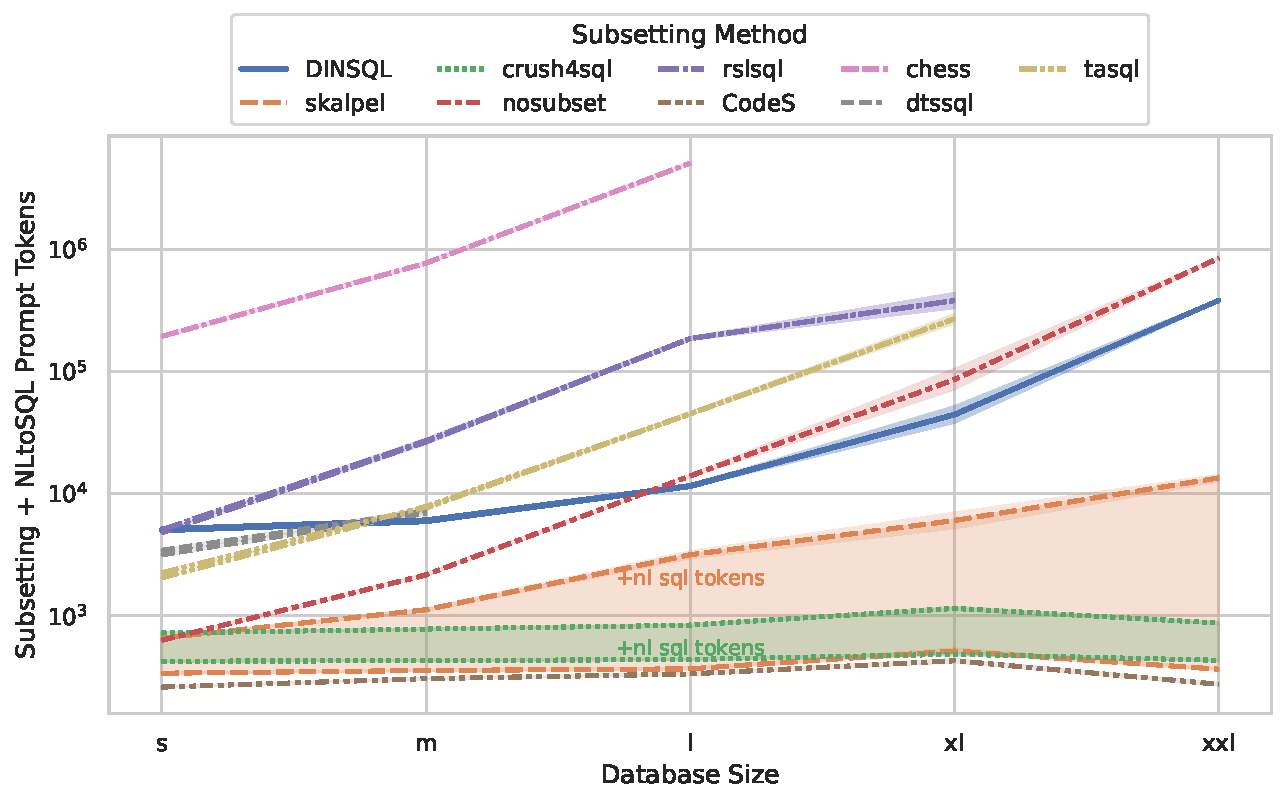
\includegraphics[width=\linewidth]{figures/combined_tokens_by_db_size_linechart.pdf}
  \caption{This chart displays total token (subsetting prompt tokens + NL-to-SQL prompt tokens) usage along the Y-axis ($log_{10}$ of prompt tokens) and database size as defined in Table~\ref{tab:benchmark-schema-sizes}. Except for Crush and \PROJECTNAME, the subsetting task dominates token usage to the point where NL-to-SQL prompt tokens are not visible. The filled area between the Crush and \PROJECTNAME{ }lines represent the additional tokens required for NL-to-SQL prompts, where the lower line represents subsetting tokens and the space between the lower and upper line represents the NL-to-SQL prompt tokens.}
  \label{fig:tokens-by-dbsize}
\end{figure}

Token usage is a cost driver for LLM-based systems either in terms of costs incurred through API transactions with LLM providers or as a surrogate for power consumption in self-hosted LLMs.
Thus, the economnic use of LLMs necessitates the monitoring of token usage and motivates the discovery of methods that achieve performance objectives while minimizing token requirements.

In Figure~\ref{fig:tokens-by-dbsize} we see that token usage varies considerably by method, and all LLM-based methods consume more tokens than simply using the full schema for NL-to-SQL over small and medium databases.
DIN SQL is the sole LLM-based method that consumes fewer tokens for large, and larger, databases, whereas other LLM-based methods continue increasing in excess of full schema NL-to-SQL prompting.

The most token-efficient LLM-based methods are the Crush subsetting method and our own \PROJECTNAME{ }prototype which use an LLM only to either hallucinate a schema or decompose an NL question without referencing the target database schema. 
While both of these hybrid methods do not exhibit a subsetting prompt token growth correlation with database size, token usage from resulting higher schema proportions and subsequent larger NL-to-SQL prompts does cause some token usage increase during NL-to-SQL inference.
Nevertheless, both Crush and \PROJECTNAME{ }consume fewer tokens than all LLM-based methods as well as full schema NL-to-SQL prompting.
CHESS expends the highest number of tokens primarily during its column selection phase which issues an LLM prompt for every column in a schema to determine the column's relevance to the NL question, a method that yields high precision scores on small, medium, and large schemas.

\subsection{Experiment 2: NL-to-SQL Performance}

\begin{figure*}
  \centering
  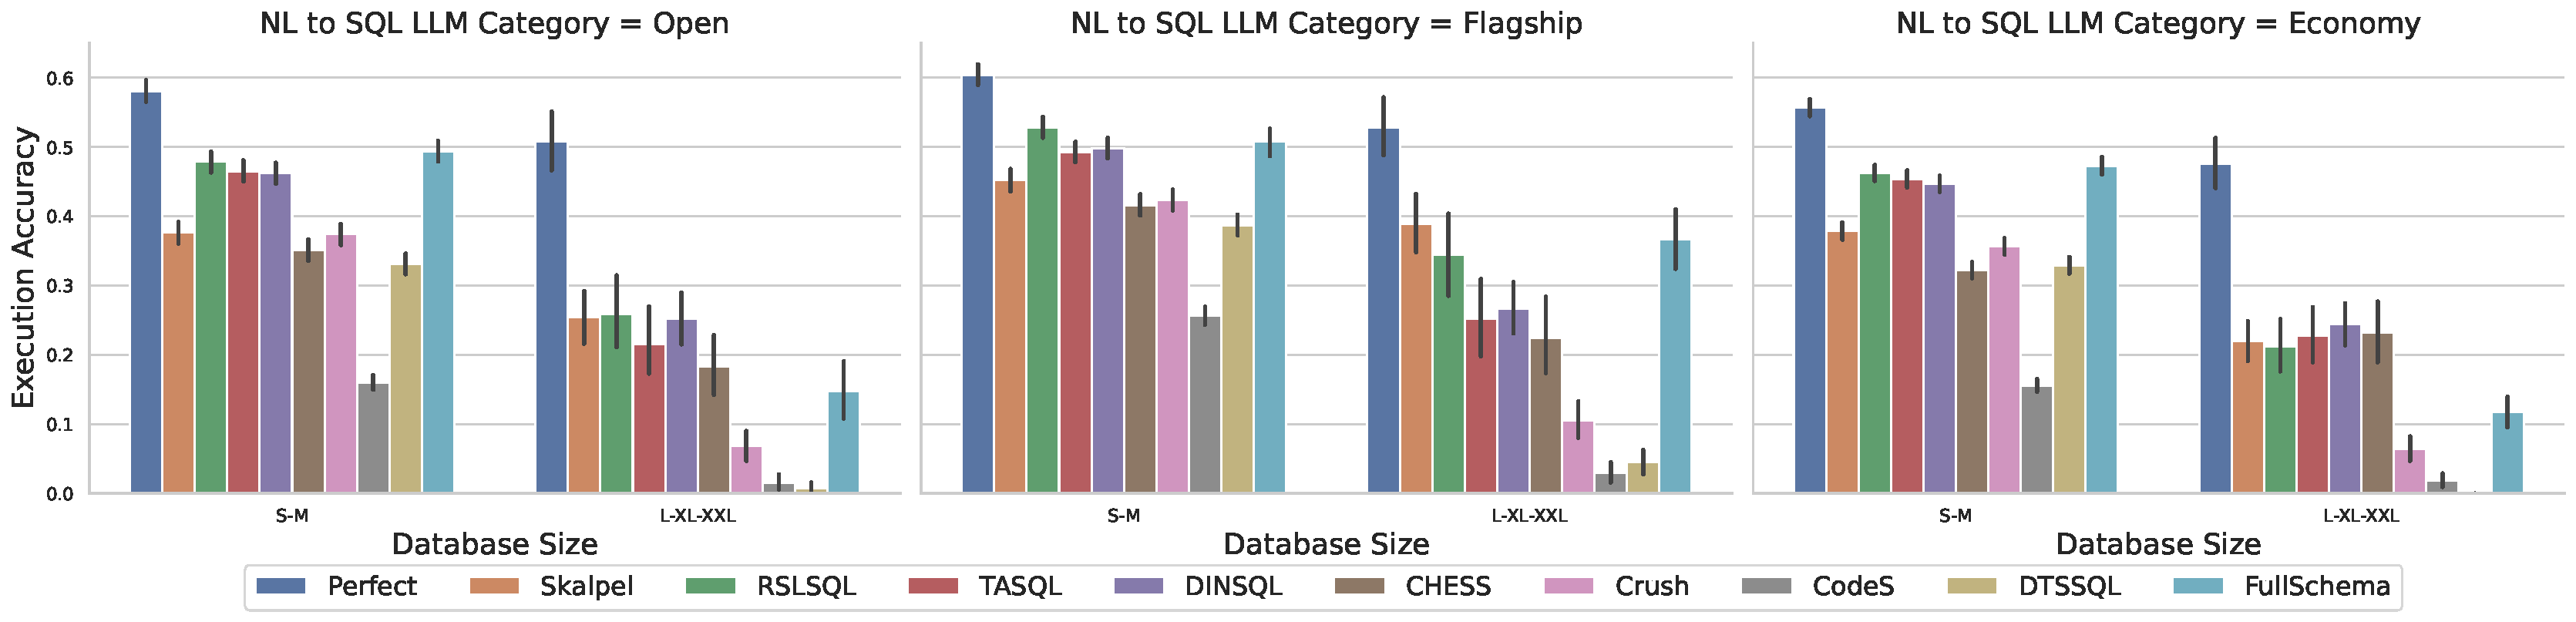
\includegraphics[width=\linewidth]{figures/nlsql_execution_accuracy_barchart_compact.pdf}
  \caption{Without considering schema size, in aggregate all subsetting methods underperform vs. full schemas on NL-to-SQL execution accuracy. We discover that subsetting effects on execution accuracy (y-axis) are schema size-dependent (x-axis). Here, we bin schema sizes into two categories (s-m, and l+ which includes l, xl, and XXL categories), and we categorize flagship models (GPT-4.1, Gemini-2.5-Pro), economy models (GPT-4.1-nano, Gemini-2.5-Flash/Flash-Lite), and open source models (Llama 3.3, GPT-OSS).}
  \label{fig:nlsqlbarchart}
\end{figure*}



\paragraph{\textbf{Subsetting Metric Effects on Execution Accuracy}}
In the results of experiment 1, we are presented with a broad array of performance measures with an equally broad variety of results across subsetting methods and schema sizes.
To determine the importance of each metric, we test correlations between the dependent variable NL-to-SQL execution accuracy and various performance measures from experiment 1.
Many performance measure independent variables exhibit a high degree of covariance (e.g., f1 is derived from precision and recall, table and column recall are highly correlated, etc.), so we use a subset of all outputs from experiment 1 as coefficients in a logistic regression model over NL-to-SQL generation attempts over subsets generated by the evaluated subsetting methods (excluding perfect subsets and full schema attempts).


Table~\ref{tab:executionaccuracycorrelations} indicates that there are significant correlations between the independent measures of \emph{TableRecall}, \emph{ColumnRecall}, and \emph{SubsetTableProportion}. 
Precision- and proportion-based independent variables indicate a statistically significant, albeit weaker, correlation to execution accuracy.
As expected, identifier recall is the prime measure of subset method performance evaluation. 
Precision is a secondary measure that should be used to differentiate subsetting methods that achieve relatively equal levels of table and column recall. 

\paragraph{\textbf{Execution Accuracy Differences Between Schema Sizes}}

Figure~\ref{fig:nlsqlbarchart} shows \emph{Execution Accuracy} for each subsetting method, a perfect subsetter, and a full schema (no subset) for two size categories of databases: small-to-medium (S-M), and large+ (L+, including L, XL, and XXL) whose labelling is consistent with the definitions in Table~\ref{tab:benchmark-schema-sizes}.
For small-to-medium sized schemas, only one method (RSLSQL + Flagship LLM) improves performance over full schema use; this holds for all categories of LLM (Open, Flagship, and Economy). 
Given the token usage comparisons (see Figure ~\ref{fig:tokens-by-dbsize}), it is safe to conclude that, with one exception (RSLSQL with a flagship LLM), none of the schema subsetters improve execution accuracy \emph{or} efficiency.
Instead, for small ane medium schemas (fewer than 1,000 columns), it is better to simply perform NL-to-SQL inference with a full schema representation.

Because we have extended subsetting analysis beyond the Bird benchmark onto the much larger Spider2 and Snails benchmarks, we can now see that for much larger schemas, both Open and Economy models benefit from RSLSQL, TASQL, DINSQL, \PROJECTNAME, and CHESS subsetting methods during NL-to-SQL inference.
Of these methods, \PROJECTNAME{ }performs at the same level as (Open LLMs), slightly better than (Flagship LLMs), or slightly under (Economy LLMs) the LLM-based methods that require a much higher number of tokens.
In the case of larger schemas (more than 1,000 columns), we find that schema subsetting \emph{can be} beneficial in terms of both execution \emph{and potentially} token efficiency given the right subsetting method and NL-to-SQL LLM category.

\begin{table}
\caption{Logistic regression coefficients, standard error, and significance (p value) for non-colinear parameters with execution accuracy as the dependent variable. n = 10,241, Pseudo R-squared = 0.099. Execution accuracy is binary (1, 0) where 1 indicates a correct NL-to-SQL generation given a schema subset.}
\label{tab:executionaccuracycorrelations}
\begin{tabular}{lccc}
\toprule
Metric & Coef & StdErr & pValue \\
\midrule
Const & -4.679 & 0.151 & 0.000 \\
TableRecall & 1.107 & 0.213 & 0.000 \\
TablePrecision & 0.599 & 0.181 & 0.001 \\
ColumnRecall & 0.933 & 0.175 & 0.000 \\
ColumnPrecision & 0.597 & 0.190 & 0.002 \\
SubsetTableProportion & -0.055 & 0.163 & 0.736 \\
SubsetColumnProportion & 0.189 & 0.217 & 0.383 \\
\bottomrule
\end{tabular}
\end{table}



\section{Discussion and Limitations}


\subsection{Discussion}

\paragraph{\textbf{Subsetting Usefulness}}
Contemporary research expresses mixed results around the usefulness of schema subsetting, and in our work we expose some of the underlying reasons for these inconstencies: namely that subsetting performance--as well as downstream NL-to-SQL inference--is database dependent, where schema size plays a large role in subsetting effectiveness and usefulness.
From our analysis, we determine that subsetting small and medium schemas (less than 1,000 columns) actually tends to worsen NL-to-SQL performance for all types of LLMs, and so we recommend full schema representations in these cases, at least until real-world schema subsetting modules can improve recall.

A case can be made for subsetting when dealing with schemas that have more than 1,000 columns. 
This is because we see that for both open source and economy LLMs NL-to-SQL execution accuracy improves when using the LLM-based subsetters (e.g., RSLSQL, TASQL, DINSQL).
In these cases, the decision to subset, and which subsetter to use, is more nuanced and depends on the tradeoff between performance and token usage.
Alternatively, our prototype \PROJECTNAME{ }hybrid subsetter offers a solution that has the potential to reduce token usage while maintaining execution accuracy at the same levels as LLM-based subsetters.

\paragraph{\textbf{Future Research}}
In this paper we refine the idea of a hybrid subsetter using LLM-aided question decomposition, LLM-generated table descriptions, and semantic search (cosine distance) to retrieve schema tables that align to the decomposed natural language questions.
Although we performed some preliminary distance search tuning based on the competing goals of high recall and reduced schema proportion, additional work can be done to identify additional ways to improve schema recall without negating the benefit of reduce schema sizes. 
Specifically, would the join path detection method in~\cite{Katsogiannis-Meimarakis2026} be an effective way to mitigate the hidden relation problem that \PROJECTNAME{ }is sensitive to?

\subsection{Limitations}

\paragraph{\textbf{Schema Size NL-to-SQL Question Distributions}}
Although, to our knowledge, this is the first work to evaluate subsetting over very large database schemas, the majority of L-, XL-, and XXL-sized schemas come from the Spider 2 benchmark, which only comprises 221 of the 2,258 total NL-to-SQL questions across all 3 benchmarks.
SNAILS provides 100 additional NL-to-SQL questions over its XXL-sized database.
Future research into subsetting over very large schemas would benefit from an increased question pool of NL-SQL question query pairs over very large schemas.

% \paragraph{\textbf{Prototype Status of the \PROJECTNAME{ }Subsetter}}
% While the results of the \PROJECTNAME{ }subsetting approach appear promising, we temper these observations by acknowledging that we derived the approach using insights from the same data and analysis that the real-world subsetting methods are exposed to and generate through experimentation.
% Thus, an unbiased evaluation using additional data would be necessary to determine if the \PROJECTNAME{ }subsetter performs better in terms of recall, precision, and f1. 
% Nevertheless, we find the preliminary results promising and suggest a further evaluation of the approach as future research.


\section{Related Work}


\paragraph{\textbf{Evaluating Schema Subsetting Methods}}
CRUSH~\cite{kothyari-etal-2023-crush4sql} is a recent work that performs subsetting evaluation of a novel halucination-based subsetting method and compares it to variations of dense passage retrieval.
The authors provide benchmark datasets including SpiderUnion, and BirdUnion--unions of the disjoint schemas in the Spider~\cite{benchmark-spider} and Bird~\cite{benchmark-bird} benchmarks respectively. They also introduce SocialDB, a collection of database schemas and schema descriptions without associated database instances and NL-SQL question-query pairs.
In our work, we extend this line of research further by adopting the  SNAILS collection to better-represent real-world schema subsetting challenges.
Additionally, we adopt a more robust benchmark evaluation strategy by introducing precision and f1 metrics in addition to the recall metric used by the CRUSH authors.
Finally, our subsetting method comparison is more representative of the current SOTA in the NL-to-SQL domain by evaluating subsetting methods described by systems with top placement on current benchmarks.

A recent ArXiv preprint that critically evaluates the usefulness of schema subsetting using SoTA LLMs suggests that as LLM capability increases, the need for schema subsetting diminishes~\cite{maamari2024deathschemalinkingtexttosql}.
In this work, the authors evaluate four LLM-based schema subsetting methods using the Bird SQL benchmark and measure performance using execution accuracy, false positive rates during subsetting, and schema linking recall.
While this concurrent work bears some resemblance to our \PROJECTNAME{ } project, we provide additional measures of recall, precision, and F1 for various combinations of table and column identifiers.
We also extend the scope of subsetting evaluation to non-LLM-based subsetting methods such as semantic similarity search- and finetuned classifier-based approaches.
In addition to the Bird benchmark, we also evaluate SoTA linking methods using the Spider2 and SNAILS benchmarks.

The authors of the \emph{In-depth Analysis of LLM-based Schema Linking}~\cite{Katsogiannis-Meimarakis2026} concurrently and independently developed a schema subsetting (or schema linking) evaluation methodology focused on LLM-based schema linking approaches in which they replicate several LLM-prompting methods for schema linking and evaluate them in terms of precision, recall, and accuracy using the Spider and Bird benchmarks~\cite{benchmark-spider,benchmark-bird}.
Our work complements this approach and makes use of the Spider 2 and SNAILS~\cite{benchmark-spider2,benchmark-snails} benchmarks which contain very large schemas.
We also opt to reproduce existing subsetting methods using original code, and additionally evaluate subsetting performance in terms of token usage as well as both online inference and offline pre-processing time requirements. 


